% !TEX root = ../main.tex
% ===================== PHỤ LỤC =====================
\setcounter{section}{0}
\renewcommand\thesection{\Alph{section}.}
\renewcommand{\thefigure}{\Alph{section}.\arabic{figure}}
\renewcommand{\thetable}{\Alph{section}.\arabic{table}}
\renewcommand{\theHsection}{app.\Alph{section}}
\renewcommand{\theHfigure}{app.\thefigure}
\renewcommand{\theHtable}{app.\thetable}
\renewcommand\sectionmark[1]{\markboth{Phụ lục \Alph{section}}{Phụ lục \Alph{section}}}
\phantomsection
\addcontentsline{toc}{section}{PHỤ LỤC}

\section{LƯỢC ĐỒ THIÊN HÀ MỨC CỘT}
Phụ lục này trình bày chi tiết ở mức cột của lược đồ thiên hà ở Hình~\ref{fig:galaxy}, chia theo hai nhóm quy trình. Hai sơ đồ được sinh tự động từ \texttt{information\_schema} của bản kho đang phát hành (\texttt{scripts/make\_erd\_tikz.py}), nên tên cột và kiểu dữ liệu khớp đúng với kho. Ký hiệu: \tikz\fill[erdkey] (0,0) circle (0.075) ++(0.06,-0.02) rectangle ++(0.14,0.04); khóa chính (khóa thay thế), vòng tròn rỗng là khóa ngoại, \tikz\fill[erdnk] (0,0) circle (0.09); khóa tự nhiên từ nguồn, \tikz\fill[erdcol, rounded corners=0.5pt] (0,-0.1) rectangle (0.09,0.1); thuộc tính hoặc số đo. Đầu ``chân chim'' ở phía fact biểu diễn bản số nhiều, hai vạch ở phía dimension biểu diễn bản số đúng một. Với các fact nhiều cột, sơ đồ giữ đủ mọi khóa và lược bớt một phần số đo (ghi chú ``+ $n$ cột khác'').

\begin{figure}[p]
\centering
\resizebox{\textwidth}{!}{\begin{tikzpicture}[x=1cm, y=1cm, erdline/.style={draw=erdwire, line width=0.55pt}]
\fill[erdbg] (-0.4,0.4) rectangle (26.8,-19.6);
\fill[erdbody, rounded corners=1.5pt] (0,0) rectangle (5.6,-5.98);
\fill[erdhead] (0,0) rectangle (5.6,-0.46);
\draw[erdred, line width=0.8pt, fill=white] (0.25,-0.23) ++(0,0.1) -- ++(0.1,-0.1) -- ++(-0.1,-0.1) -- ++(-0.1,0.1) -- cycle;
\node[anchor=west, text=erdtext, font=\erdfont\scriptsize\bfseries] at (0.45,-0.23) {core};
\draw[erdtbl, line width=0.6pt] (0.17,-0.78) rectangle (0.35,-0.6000000000000001); \draw[erdtbl] (0.17,-0.66) -- (0.35,-0.66);
\node[anchor=west, text=erdtext, font=\erdfont\scriptsize\bfseries] at (0.45,-0.6900000000000001) {dim\_date};
\draw[erdgrid, line width=0.4pt] (0,-0.92) -- (5.6,-0.92);
\fill[erdkey] (0.150,-1.150) circle (0.075); \fill[erdkey] (0.150+0.06,-1.150-0.02) rectangle (0.150+0.2,-1.150+0.02);
\node[anchor=west, text=erdtext, font=\erdfont\scriptsize] at (0.45,-1.1500000000000001) {date\_key \textcolor{erdmuted}{integer}};
\draw[erdgrid, line width=0.4pt] (0,-1.3800000000000001) -- (5.6,-1.3800000000000001);
\fill[erdcol, rounded corners=0.5pt] (0.150+0.03,-1.610-0.1) rectangle (0.150+0.12,-1.610+0.1);
\node[anchor=west, text=erdtext, font=\erdfont\scriptsize] at (0.45,-1.61) {full\_date \textcolor{erdmuted}{date}};
\draw[erdgrid, line width=0.4pt] (0,-1.84) -- (5.6,-1.84);
\fill[erdcol, rounded corners=0.5pt] (0.150+0.03,-2.070-0.1) rectangle (0.150+0.12,-2.070+0.1);
\node[anchor=west, text=erdtext, font=\erdfont\scriptsize] at (0.45,-2.0700000000000003) {year \textcolor{erdmuted}{bigint}};
\draw[erdgrid, line width=0.4pt] (0,-2.3000000000000003) -- (5.6,-2.3000000000000003);
\fill[erdcol, rounded corners=0.5pt] (0.150+0.03,-2.530-0.1) rectangle (0.150+0.12,-2.530+0.1);
\node[anchor=west, text=erdtext, font=\erdfont\scriptsize] at (0.45,-2.5300000000000002) {quarter \textcolor{erdmuted}{bigint}};
\draw[erdgrid, line width=0.4pt] (0,-2.7600000000000002) -- (5.6,-2.7600000000000002);
\fill[erdcol, rounded corners=0.5pt] (0.150+0.03,-2.990-0.1) rectangle (0.150+0.12,-2.990+0.1);
\node[anchor=west, text=erdtext, font=\erdfont\scriptsize] at (0.45,-2.99) {month \textcolor{erdmuted}{bigint}};
\draw[erdgrid, line width=0.4pt] (0,-3.22) -- (5.6,-3.22);
\fill[erdcol, rounded corners=0.5pt] (0.150+0.03,-3.450-0.1) rectangle (0.150+0.12,-3.450+0.1);
\node[anchor=west, text=erdtext, font=\erdfont\scriptsize] at (0.45,-3.45) {year\_month \textcolor{erdmuted}{text}};
\draw[erdgrid, line width=0.4pt] (0,-3.68) -- (5.6,-3.68);
\fill[erdcol, rounded corners=0.5pt] (0.150+0.03,-3.910-0.1) rectangle (0.150+0.12,-3.910+0.1);
\node[anchor=west, text=erdtext, font=\erdfont\scriptsize] at (0.45,-3.91) {week \textcolor{erdmuted}{bigint}};
\draw[erdgrid, line width=0.4pt] (0,-4.140000000000001) -- (5.6,-4.140000000000001);
\fill[erdcol, rounded corners=0.5pt] (0.150+0.03,-4.370-0.1) rectangle (0.150+0.12,-4.370+0.1);
\node[anchor=west, text=erdtext, font=\erdfont\scriptsize] at (0.45,-4.370000000000001) {day\_of\_week \textcolor{erdmuted}{bigint}};
\draw[erdgrid, line width=0.4pt] (0,-4.6000000000000005) -- (5.6,-4.6000000000000005);
\fill[erdcol, rounded corners=0.5pt] (0.150+0.03,-4.830-0.1) rectangle (0.150+0.12,-4.830+0.1);
\node[anchor=west, text=erdtext, font=\erdfont\scriptsize] at (0.45,-4.830000000000001) {is\_weekend \textcolor{erdmuted}{boolean}};
\draw[erdgrid, line width=0.4pt] (0,-5.0600000000000005) -- (5.6,-5.0600000000000005);
\fill[erdcol, rounded corners=0.5pt] (0.150+0.03,-5.290-0.1) rectangle (0.150+0.12,-5.290+0.1);
\node[anchor=west, text=erdtext, font=\erdfont\scriptsize] at (0.45,-5.290000000000001) {is\_holiday\_br \textcolor{erdmuted}{boolean}};
\draw[erdgrid, line width=0.4pt] (0,-5.5200000000000005) -- (5.6,-5.5200000000000005);
\fill[erdcol, rounded corners=0.5pt] (0.150+0.03,-5.750-0.1) rectangle (0.150+0.12,-5.750+0.1);
\node[anchor=west, text=erdtext, font=\erdfont\scriptsize] at (0.45,-5.750000000000001) {is\_black\_friday \textcolor{erdmuted}{boolean}};
\draw[erdborder, line width=0.6pt, rounded corners=1.5pt] (0,0) rectangle (5.6,-5.98);
\fill[erdbody, rounded corners=1.5pt] (0,-7.2) rectangle (5.6,-9.96);
\fill[erdhead] (0,-7.2) rectangle (5.6,-7.66);
\draw[erdred, line width=0.8pt, fill=white] (0.25,-7.430000000000001) ++(0,0.1) -- ++(0.1,-0.1) -- ++(-0.1,-0.1) -- ++(-0.1,0.1) -- cycle;
\node[anchor=west, text=erdtext, font=\erdfont\scriptsize\bfseries] at (0.45,-7.430000000000001) {core};
\draw[erdtbl, line width=0.6pt] (0.17,-7.98) rectangle (0.35,-7.800000000000001); \draw[erdtbl] (0.17,-7.86) -- (0.35,-7.86);
\node[anchor=west, text=erdtext, font=\erdfont\scriptsize\bfseries] at (0.45,-7.890000000000001) {dim\_customer};
\draw[erdgrid, line width=0.4pt] (0,-8.120000000000001) -- (5.6,-8.120000000000001);
\fill[erdkey] (0.150,-8.350) circle (0.075); \fill[erdkey] (0.150+0.06,-8.350-0.02) rectangle (0.150+0.2,-8.350+0.02);
\node[anchor=west, text=erdtext, font=\erdfont\scriptsize] at (0.45,-8.350000000000001) {customer\_key \textcolor{erdmuted}{bigint}};
\draw[erdgrid, line width=0.4pt] (0,-8.58) -- (5.6,-8.58);
\fill[erdnk] (0.150+0.07,-8.810) circle (0.09); \node[text=white, font=\erdfont\fontsize{4}{4}\selectfont] at (0.150+0.07,-8.810) {1};
\node[anchor=west, text=erdtext, font=\erdfont\scriptsize] at (0.45,-8.81) {customer\_unique\_id \textcolor{erdmuted}{text}};
\draw[erdgrid, line width=0.4pt] (0,-9.040000000000001) -- (5.6,-9.040000000000001);
\fill[erdcol, rounded corners=0.5pt] (0.150+0.03,-9.270-0.1) rectangle (0.150+0.12,-9.270+0.1);
\node[anchor=west, text=erdtext, font=\erdfont\scriptsize] at (0.45,-9.270000000000001) {city \textcolor{erdmuted}{text}};
\draw[erdgrid, line width=0.4pt] (0,-9.5) -- (5.6,-9.5);
\fill[erdcol, rounded corners=0.5pt] (0.150+0.03,-9.730-0.1) rectangle (0.150+0.12,-9.730+0.1);
\node[anchor=west, text=erdtext, font=\erdfont\scriptsize] at (0.45,-9.73) {state \textcolor{erdmuted}{text}};
\draw[erdborder, line width=0.6pt, rounded corners=1.5pt] (0,-7.2) rectangle (5.6,-9.96);
\fill[erdbody, rounded corners=1.5pt] (0,-10.4) rectangle (5.6,-15.0);
\fill[erdhead] (0,-10.4) rectangle (5.6,-10.860000000000001);
\draw[erdred, line width=0.8pt, fill=white] (0.25,-10.63) ++(0,0.1) -- ++(0.1,-0.1) -- ++(-0.1,-0.1) -- ++(-0.1,0.1) -- cycle;
\node[anchor=west, text=erdtext, font=\erdfont\scriptsize\bfseries] at (0.45,-10.63) {core};
\draw[erdtbl, line width=0.6pt] (0.17,-11.18) rectangle (0.35,-11.0); \draw[erdtbl] (0.17,-11.06) -- (0.35,-11.06);
\node[anchor=west, text=erdtext, font=\erdfont\scriptsize\bfseries] at (0.45,-11.09) {dim\_location};
\draw[erdgrid, line width=0.4pt] (0,-11.32) -- (5.6,-11.32);
\fill[erdkey] (0.150,-11.550) circle (0.075); \fill[erdkey] (0.150+0.06,-11.550-0.02) rectangle (0.150+0.2,-11.550+0.02);
\node[anchor=west, text=erdtext, font=\erdfont\scriptsize] at (0.45,-11.55) {location\_key \textcolor{erdmuted}{bigint}};
\draw[erdgrid, line width=0.4pt] (0,-11.780000000000001) -- (5.6,-11.780000000000001);
\fill[erdnk] (0.150+0.07,-12.010) circle (0.09); \node[text=white, font=\erdfont\fontsize{4}{4}\selectfont] at (0.150+0.07,-12.010) {1};
\node[anchor=west, text=erdtext, font=\erdfont\scriptsize] at (0.45,-12.010000000000002) {zip\_prefix \textcolor{erdmuted}{text}};
\draw[erdgrid, line width=0.4pt] (0,-12.24) -- (5.6,-12.24);
\fill[erdcol, rounded corners=0.5pt] (0.150+0.03,-12.470-0.1) rectangle (0.150+0.12,-12.470+0.1);
\node[anchor=west, text=erdtext, font=\erdfont\scriptsize] at (0.45,-12.47) {city \textcolor{erdmuted}{text}};
\draw[erdgrid, line width=0.4pt] (0,-12.700000000000001) -- (5.6,-12.700000000000001);
\fill[erdcol, rounded corners=0.5pt] (0.150+0.03,-12.930-0.1) rectangle (0.150+0.12,-12.930+0.1);
\node[anchor=west, text=erdtext, font=\erdfont\scriptsize] at (0.45,-12.930000000000001) {state \textcolor{erdmuted}{text}};
\draw[erdgrid, line width=0.4pt] (0,-13.16) -- (5.6,-13.16);
\fill[erdcol, rounded corners=0.5pt] (0.150+0.03,-13.390-0.1) rectangle (0.150+0.12,-13.390+0.1);
\node[anchor=west, text=erdtext, font=\erdfont\scriptsize] at (0.45,-13.39) {region \textcolor{erdmuted}{text}};
\draw[erdgrid, line width=0.4pt] (0,-13.620000000000001) -- (5.6,-13.620000000000001);
\fill[erdcol, rounded corners=0.5pt] (0.150+0.03,-13.850-0.1) rectangle (0.150+0.12,-13.850+0.1);
\node[anchor=west, text=erdtext, font=\erdfont\scriptsize] at (0.45,-13.850000000000001) {lat \textcolor{erdmuted}{double}};
\draw[erdgrid, line width=0.4pt] (0,-14.08) -- (5.6,-14.08);
\fill[erdcol, rounded corners=0.5pt] (0.150+0.03,-14.310-0.1) rectangle (0.150+0.12,-14.310+0.1);
\node[anchor=west, text=erdtext, font=\erdfont\scriptsize] at (0.45,-14.31) {lng \textcolor{erdmuted}{double}};
\draw[erdgrid, line width=0.4pt] (0,-14.540000000000001) -- (5.6,-14.540000000000001);
\fill[erdcol, rounded corners=0.5pt] (0.150+0.03,-14.770-0.1) rectangle (0.150+0.12,-14.770+0.1);
\node[anchor=west, text=erdtext, font=\erdfont\scriptsize] at (0.45,-14.770000000000001) {has\_coordinates \textcolor{erdmuted}{boolean}};
\draw[erdborder, line width=0.6pt, rounded corners=1.5pt] (0,-10.4) rectangle (5.6,-15.0);
\fill[erdbody, rounded corners=1.5pt] (10.4,0) rectangle (16.0,-8.74);
\fill[erdhead] (10.4,0) rectangle (16.0,-0.46);
\draw[erdred, line width=0.8pt, fill=white] (10.65,-0.23) ++(0,0.1) -- ++(0.1,-0.1) -- ++(-0.1,-0.1) -- ++(-0.1,0.1) -- cycle;
\node[anchor=west, text=erdtext, font=\erdfont\scriptsize\bfseries] at (10.85,-0.23) {core};
\draw[erdtbl, line width=0.6pt] (10.57,-0.78) rectangle (10.75,-0.6000000000000001); \draw[erdtbl] (10.57,-0.66) -- (10.75,-0.66);
\node[anchor=west, text=erdtext, font=\erdfont\scriptsize\bfseries] at (10.85,-0.6900000000000001) {fact\_sales\_item};
\draw[erdgrid, line width=0.4pt] (10.4,-0.92) -- (16.0,-0.92);
\fill[erdnk] (10.550+0.07,-1.150) circle (0.09); \node[text=white, font=\erdfont\fontsize{4}{4}\selectfont] at (10.550+0.07,-1.150) {1};
\node[anchor=west, text=erdtext, font=\erdfont\scriptsize] at (10.85,-1.1500000000000001) {order\_id \textcolor{erdmuted}{text}};
\draw[erdgrid, line width=0.4pt] (10.4,-1.3800000000000001) -- (16.0,-1.3800000000000001);
\fill[erdcol, rounded corners=0.5pt] (10.550+0.03,-1.610-0.1) rectangle (10.550+0.12,-1.610+0.1);
\node[anchor=west, text=erdtext, font=\erdfont\scriptsize] at (10.85,-1.61) {order\_item\_id \textcolor{erdmuted}{integer}};
\draw[erdgrid, line width=0.4pt] (10.4,-1.84) -- (16.0,-1.84);
\draw[erdfk, line width=0.7pt] (10.550,-2.070) circle (0.07); \draw[erdfk, line width=0.7pt] (10.550+0.07,-2.070) -- (10.550+0.2,-2.070);
\node[anchor=west, text=erdtext, font=\erdfont\scriptsize] at (10.85,-2.0700000000000003) {product\_key \textcolor{erdmuted}{bigint}};
\draw[erdgrid, line width=0.4pt] (10.4,-2.3000000000000003) -- (16.0,-2.3000000000000003);
\draw[erdfk, line width=0.7pt] (10.550,-2.530) circle (0.07); \draw[erdfk, line width=0.7pt] (10.550+0.07,-2.530) -- (10.550+0.2,-2.530);
\node[anchor=west, text=erdtext, font=\erdfont\scriptsize] at (10.85,-2.5300000000000002) {seller\_key \textcolor{erdmuted}{bigint}};
\draw[erdgrid, line width=0.4pt] (10.4,-2.7600000000000002) -- (16.0,-2.7600000000000002);
\fill[erdnk] (10.550+0.07,-2.990) circle (0.09); \node[text=white, font=\erdfont\fontsize{4}{4}\selectfont] at (10.550+0.07,-2.990) {1};
\node[anchor=west, text=erdtext, font=\erdfont\scriptsize] at (10.85,-2.99) {seller\_id \textcolor{erdmuted}{text}};
\draw[erdgrid, line width=0.4pt] (10.4,-3.22) -- (16.0,-3.22);
\draw[erdfk, line width=0.7pt] (10.550,-3.450) circle (0.07); \draw[erdfk, line width=0.7pt] (10.550+0.07,-3.450) -- (10.550+0.2,-3.450);
\node[anchor=west, text=erdtext, font=\erdfont\scriptsize] at (10.85,-3.45) {customer\_key \textcolor{erdmuted}{bigint}};
\draw[erdgrid, line width=0.4pt] (10.4,-3.68) -- (16.0,-3.68);
\draw[erdfk, line width=0.7pt] (10.550,-3.910) circle (0.07); \draw[erdfk, line width=0.7pt] (10.550+0.07,-3.910) -- (10.550+0.2,-3.910);
\node[anchor=west, text=erdtext, font=\erdfont\scriptsize] at (10.85,-3.91) {route\_key \textcolor{erdmuted}{bigint}};
\draw[erdgrid, line width=0.4pt] (10.4,-4.140000000000001) -- (16.0,-4.140000000000001);
\draw[erdfk, line width=0.7pt] (10.550,-4.370) circle (0.07); \draw[erdfk, line width=0.7pt] (10.550+0.07,-4.370) -- (10.550+0.2,-4.370);
\node[anchor=west, text=erdtext, font=\erdfont\scriptsize] at (10.85,-4.370000000000001) {customer\_location\_key \textcolor{erdmuted}{bigint}};
\draw[erdgrid, line width=0.4pt] (10.4,-4.6000000000000005) -- (16.0,-4.6000000000000005);
\draw[erdfk, line width=0.7pt] (10.550,-4.830) circle (0.07); \draw[erdfk, line width=0.7pt] (10.550+0.07,-4.830) -- (10.550+0.2,-4.830);
\node[anchor=west, text=erdtext, font=\erdfont\scriptsize] at (10.85,-4.830000000000001) {seller\_location\_key \textcolor{erdmuted}{bigint}};
\draw[erdgrid, line width=0.4pt] (10.4,-5.0600000000000005) -- (16.0,-5.0600000000000005);
\draw[erdfk, line width=0.7pt] (10.550,-5.290) circle (0.07); \draw[erdfk, line width=0.7pt] (10.550+0.07,-5.290) -- (10.550+0.2,-5.290);
\node[anchor=west, text=erdtext, font=\erdfont\scriptsize] at (10.85,-5.290000000000001) {purchase\_date\_key \textcolor{erdmuted}{integer}};
\draw[erdgrid, line width=0.4pt] (10.4,-5.5200000000000005) -- (16.0,-5.5200000000000005);
\draw[erdfk, line width=0.7pt] (10.550,-5.750) circle (0.07); \draw[erdfk, line width=0.7pt] (10.550+0.07,-5.750) -- (10.550+0.2,-5.750);
\node[anchor=west, text=erdtext, font=\erdfont\scriptsize] at (10.85,-5.750000000000001) {shipping\_limit\_date\_key \textcolor{erdmuted}{integer}};
\draw[erdgrid, line width=0.4pt] (10.4,-5.98) -- (16.0,-5.98);
\fill[erdcol, rounded corners=0.5pt] (10.550+0.03,-6.210-0.1) rectangle (10.550+0.12,-6.210+0.1);
\node[anchor=west, text=erdtext, font=\erdfont\scriptsize] at (10.85,-6.210000000000001) {purchase\_ts \textcolor{erdmuted}{timestamp}};
\draw[erdgrid, line width=0.4pt] (10.4,-6.44) -- (16.0,-6.44);
\fill[erdcol, rounded corners=0.5pt] (10.550+0.03,-6.670-0.1) rectangle (10.550+0.12,-6.670+0.1);
\node[anchor=west, text=erdtext, font=\erdfont\scriptsize] at (10.85,-6.670000000000001) {shipping\_limit\_ts \textcolor{erdmuted}{timestamp}};
\draw[erdgrid, line width=0.4pt] (10.4,-6.9) -- (16.0,-6.9);
\fill[erdcol, rounded corners=0.5pt] (10.550+0.03,-7.130-0.1) rectangle (10.550+0.12,-7.130+0.1);
\node[anchor=west, text=erdtext, font=\erdfont\scriptsize] at (10.85,-7.130000000000001) {price \textcolor{erdmuted}{decimal(12,2)}};
\draw[erdgrid, line width=0.4pt] (10.4,-7.36) -- (16.0,-7.36);
\fill[erdcol, rounded corners=0.5pt] (10.550+0.03,-7.590-0.1) rectangle (10.550+0.12,-7.590+0.1);
\node[anchor=west, text=erdtext, font=\erdfont\scriptsize] at (10.85,-7.590000000000001) {freight\_value \textcolor{erdmuted}{decimal(12,2)}};
\draw[erdgrid, line width=0.4pt] (10.4,-7.82) -- (16.0,-7.82);
\fill[erdcol, rounded corners=0.5pt] (10.550+0.03,-8.050-0.1) rectangle (10.550+0.12,-8.050+0.1);
\node[anchor=west, text=erdtext, font=\erdfont\scriptsize] at (10.85,-8.05) {qty \textcolor{erdmuted}{integer}};
\draw[erdgrid, line width=0.4pt] (10.4,-8.280000000000001) -- (16.0,-8.280000000000001);
\fill[erdcol, rounded corners=0.5pt] (10.550+0.03,-8.510-0.1) rectangle (10.550+0.12,-8.510+0.1);
\node[anchor=west, text=erdtext, font=\erdfont\scriptsize] at (10.85,-8.510000000000002) {is\_valid\_sale \textcolor{erdmuted}{boolean}};
\draw[erdborder, line width=0.6pt, rounded corners=1.5pt] (10.4,0) rectangle (16.0,-8.74);
\fill[erdbody, rounded corners=1.5pt] (10.4,-9.6) rectangle (16.0,-18.8);
\fill[erdhead] (10.4,-9.6) rectangle (16.0,-10.06);
\draw[erdred, line width=0.8pt, fill=white] (10.65,-9.83) ++(0,0.1) -- ++(0.1,-0.1) -- ++(-0.1,-0.1) -- ++(-0.1,0.1) -- cycle;
\node[anchor=west, text=erdtext, font=\erdfont\scriptsize\bfseries] at (10.85,-9.83) {core};
\draw[erdtbl, line width=0.6pt] (10.57,-10.379999999999999) rectangle (10.75,-10.2); \draw[erdtbl] (10.57,-10.26) -- (10.75,-10.26);
\node[anchor=west, text=erdtext, font=\erdfont\scriptsize\bfseries] at (10.85,-10.29) {fact\_order\_seller};
\draw[erdgrid, line width=0.4pt] (10.4,-10.52) -- (16.0,-10.52);
\fill[erdnk] (10.550+0.07,-10.750) circle (0.09); \node[text=white, font=\erdfont\fontsize{4}{4}\selectfont] at (10.550+0.07,-10.750) {1};
\node[anchor=west, text=erdtext, font=\erdfont\scriptsize] at (10.85,-10.75) {order\_id \textcolor{erdmuted}{text}};
\draw[erdgrid, line width=0.4pt] (10.4,-10.98) -- (16.0,-10.98);
\fill[erdnk] (10.550+0.07,-11.210) circle (0.09); \node[text=white, font=\erdfont\fontsize{4}{4}\selectfont] at (10.550+0.07,-11.210) {1};
\node[anchor=west, text=erdtext, font=\erdfont\scriptsize] at (10.85,-11.21) {seller\_id \textcolor{erdmuted}{text}};
\draw[erdgrid, line width=0.4pt] (10.4,-11.44) -- (16.0,-11.44);
\draw[erdfk, line width=0.7pt] (10.550,-11.670) circle (0.07); \draw[erdfk, line width=0.7pt] (10.550+0.07,-11.670) -- (10.550+0.2,-11.670);
\node[anchor=west, text=erdtext, font=\erdfont\scriptsize] at (10.85,-11.67) {seller\_key \textcolor{erdmuted}{bigint}};
\draw[erdgrid, line width=0.4pt] (10.4,-11.9) -- (16.0,-11.9);
\draw[erdfk, line width=0.7pt] (10.550,-12.130) circle (0.07); \draw[erdfk, line width=0.7pt] (10.550+0.07,-12.130) -- (10.550+0.2,-12.130);
\node[anchor=west, text=erdtext, font=\erdfont\scriptsize] at (10.85,-12.13) {customer\_key \textcolor{erdmuted}{bigint}};
\draw[erdgrid, line width=0.4pt] (10.4,-12.36) -- (16.0,-12.36);
\draw[erdfk, line width=0.7pt] (10.550,-12.590) circle (0.07); \draw[erdfk, line width=0.7pt] (10.550+0.07,-12.590) -- (10.550+0.2,-12.590);
\node[anchor=west, text=erdtext, font=\erdfont\scriptsize] at (10.85,-12.59) {route\_key \textcolor{erdmuted}{bigint}};
\draw[erdgrid, line width=0.4pt] (10.4,-12.82) -- (16.0,-12.82);
\draw[erdfk, line width=0.7pt] (10.550,-13.050) circle (0.07); \draw[erdfk, line width=0.7pt] (10.550+0.07,-13.050) -- (10.550+0.2,-13.050);
\node[anchor=west, text=erdtext, font=\erdfont\scriptsize] at (10.85,-13.05) {customer\_location\_key \textcolor{erdmuted}{bigint}};
\draw[erdgrid, line width=0.4pt] (10.4,-13.28) -- (16.0,-13.28);
\draw[erdfk, line width=0.7pt] (10.550,-13.510) circle (0.07); \draw[erdfk, line width=0.7pt] (10.550+0.07,-13.510) -- (10.550+0.2,-13.510);
\node[anchor=west, text=erdtext, font=\erdfont\scriptsize] at (10.85,-13.51) {seller\_location\_key \textcolor{erdmuted}{bigint}};
\draw[erdgrid, line width=0.4pt] (10.4,-13.74) -- (16.0,-13.74);
\draw[erdfk, line width=0.7pt] (10.550,-13.970) circle (0.07); \draw[erdfk, line width=0.7pt] (10.550+0.07,-13.970) -- (10.550+0.2,-13.970);
\node[anchor=west, text=erdtext, font=\erdfont\scriptsize] at (10.85,-13.97) {purchase\_date\_key \textcolor{erdmuted}{integer}};
\draw[erdgrid, line width=0.4pt] (10.4,-14.2) -- (16.0,-14.2);
\draw[erdfk, line width=0.7pt] (10.550,-14.430) circle (0.07); \draw[erdfk, line width=0.7pt] (10.550+0.07,-14.430) -- (10.550+0.2,-14.430);
\node[anchor=west, text=erdtext, font=\erdfont\scriptsize] at (10.85,-14.43) {approved\_date\_key \textcolor{erdmuted}{integer}};
\draw[erdgrid, line width=0.4pt] (10.4,-14.66) -- (16.0,-14.66);
\draw[erdfk, line width=0.7pt] (10.550,-14.890) circle (0.07); \draw[erdfk, line width=0.7pt] (10.550+0.07,-14.890) -- (10.550+0.2,-14.890);
\node[anchor=west, text=erdtext, font=\erdfont\scriptsize] at (10.85,-14.89) {carrier\_date\_key \textcolor{erdmuted}{integer}};
\draw[erdgrid, line width=0.4pt] (10.4,-15.120000000000001) -- (16.0,-15.120000000000001);
\draw[erdfk, line width=0.7pt] (10.550,-15.350) circle (0.07); \draw[erdfk, line width=0.7pt] (10.550+0.07,-15.350) -- (10.550+0.2,-15.350);
\node[anchor=west, text=erdtext, font=\erdfont\scriptsize] at (10.85,-15.350000000000001) {delivered\_date\_key \textcolor{erdmuted}{integer}};
\draw[erdgrid, line width=0.4pt] (10.4,-15.58) -- (16.0,-15.58);
\draw[erdfk, line width=0.7pt] (10.550,-15.810) circle (0.07); \draw[erdfk, line width=0.7pt] (10.550+0.07,-15.810) -- (10.550+0.2,-15.810);
\node[anchor=west, text=erdtext, font=\erdfont\scriptsize] at (10.85,-15.81) {estimated\_date\_key \textcolor{erdmuted}{integer}};
\draw[erdgrid, line width=0.4pt] (10.4,-16.04) -- (16.0,-16.04);
\fill[erdcol, rounded corners=0.5pt] (10.550+0.03,-16.270-0.1) rectangle (10.550+0.12,-16.270+0.1);
\node[anchor=west, text=erdtext, font=\erdfont\scriptsize] at (10.85,-16.27) {purchase\_ts \textcolor{erdmuted}{timestamp}};
\draw[erdgrid, line width=0.4pt] (10.4,-16.5) -- (16.0,-16.5);
\fill[erdcol, rounded corners=0.5pt] (10.550+0.03,-16.730-0.1) rectangle (10.550+0.12,-16.730+0.1);
\node[anchor=west, text=erdtext, font=\erdfont\scriptsize] at (10.85,-16.73) {approved\_ts \textcolor{erdmuted}{timestamp}};
\draw[erdgrid, line width=0.4pt] (10.4,-16.96) -- (16.0,-16.96);
\fill[erdcol, rounded corners=0.5pt] (10.550+0.03,-17.190-0.1) rectangle (10.550+0.12,-17.190+0.1);
\node[anchor=west, text=erdtext, font=\erdfont\scriptsize] at (10.85,-17.19) {carrier\_ts \textcolor{erdmuted}{timestamp}};
\draw[erdgrid, line width=0.4pt] (10.4,-17.42) -- (16.0,-17.42);
\fill[erdcol, rounded corners=0.5pt] (10.550+0.03,-17.650-0.1) rectangle (10.550+0.12,-17.650+0.1);
\node[anchor=west, text=erdtext, font=\erdfont\scriptsize] at (10.85,-17.650000000000002) {delivered\_ts \textcolor{erdmuted}{timestamp}};
\draw[erdgrid, line width=0.4pt] (10.4,-17.880000000000003) -- (16.0,-17.880000000000003);
\fill[erdcol, rounded corners=0.5pt] (10.550+0.03,-18.110-0.1) rectangle (10.550+0.12,-18.110+0.1);
\node[anchor=west, text=erdtext, font=\erdfont\scriptsize] at (10.85,-18.110000000000003) {estimated\_ts \textcolor{erdmuted}{timestamp}};
\draw[erdgrid, line width=0.4pt] (10.4,-18.34) -- (16.0,-18.34);
\node[anchor=west, text=erdmuted, font=\erdfont\scriptsize\itshape] at (10.85,-18.57) {+ 14 cột khác};
\draw[erdborder, line width=0.6pt, rounded corners=1.5pt] (10.4,-9.6) rectangle (16.0,-18.8);
\fill[erdbody, rounded corners=1.5pt] (20.8,0) rectangle (26.4,-4.140000000000001);
\fill[erdhead] (20.8,0) rectangle (26.4,-0.46);
\draw[erdred, line width=0.8pt, fill=white] (21.05,-0.23) ++(0,0.1) -- ++(0.1,-0.1) -- ++(-0.1,-0.1) -- ++(-0.1,0.1) -- cycle;
\node[anchor=west, text=erdtext, font=\erdfont\scriptsize\bfseries] at (21.25,-0.23) {core};
\draw[erdtbl, line width=0.6pt] (20.970000000000002,-0.78) rectangle (21.150000000000002,-0.6000000000000001); \draw[erdtbl] (20.970000000000002,-0.66) -- (21.150000000000002,-0.66);
\node[anchor=west, text=erdtext, font=\erdfont\scriptsize\bfseries] at (21.25,-0.6900000000000001) {dim\_product};
\draw[erdgrid, line width=0.4pt] (20.8,-0.92) -- (26.4,-0.92);
\fill[erdkey] (20.950,-1.150) circle (0.075); \fill[erdkey] (20.950+0.06,-1.150-0.02) rectangle (20.950+0.2,-1.150+0.02);
\node[anchor=west, text=erdtext, font=\erdfont\scriptsize] at (21.25,-1.1500000000000001) {product\_key \textcolor{erdmuted}{bigint}};
\draw[erdgrid, line width=0.4pt] (20.8,-1.3800000000000001) -- (26.4,-1.3800000000000001);
\fill[erdnk] (20.950+0.07,-1.610) circle (0.09); \node[text=white, font=\erdfont\fontsize{4}{4}\selectfont] at (20.950+0.07,-1.610) {1};
\node[anchor=west, text=erdtext, font=\erdfont\scriptsize] at (21.25,-1.61) {product\_id \textcolor{erdmuted}{text}};
\draw[erdgrid, line width=0.4pt] (20.8,-1.84) -- (26.4,-1.84);
\fill[erdcol, rounded corners=0.5pt] (20.950+0.03,-2.070-0.1) rectangle (20.950+0.12,-2.070+0.1);
\node[anchor=west, text=erdtext, font=\erdfont\scriptsize] at (21.25,-2.0700000000000003) {category\_en \textcolor{erdmuted}{text}};
\draw[erdgrid, line width=0.4pt] (20.8,-2.3000000000000003) -- (26.4,-2.3000000000000003);
\fill[erdcol, rounded corners=0.5pt] (20.950+0.03,-2.530-0.1) rectangle (20.950+0.12,-2.530+0.1);
\node[anchor=west, text=erdtext, font=\erdfont\scriptsize] at (21.25,-2.5300000000000002) {weight\_g \textcolor{erdmuted}{double}};
\draw[erdgrid, line width=0.4pt] (20.8,-2.7600000000000002) -- (26.4,-2.7600000000000002);
\fill[erdcol, rounded corners=0.5pt] (20.950+0.03,-2.990-0.1) rectangle (20.950+0.12,-2.990+0.1);
\node[anchor=west, text=erdtext, font=\erdfont\scriptsize] at (21.25,-2.99) {volume\_cm3 \textcolor{erdmuted}{double}};
\draw[erdgrid, line width=0.4pt] (20.8,-3.22) -- (26.4,-3.22);
\fill[erdcol, rounded corners=0.5pt] (20.950+0.03,-3.450-0.1) rectangle (20.950+0.12,-3.450+0.1);
\node[anchor=west, text=erdtext, font=\erdfont\scriptsize] at (21.25,-3.45) {size\_group \textcolor{erdmuted}{text}};
\draw[erdgrid, line width=0.4pt] (20.8,-3.68) -- (26.4,-3.68);
\fill[erdcol, rounded corners=0.5pt] (20.950+0.03,-3.910-0.1) rectangle (20.950+0.12,-3.910+0.1);
\node[anchor=west, text=erdtext, font=\erdfont\scriptsize] at (21.25,-3.91) {photos\_qty \textcolor{erdmuted}{integer}};
\draw[erdborder, line width=0.6pt, rounded corners=1.5pt] (20.8,0) rectangle (26.4,-4.140000000000001);
\fill[erdbody, rounded corners=1.5pt] (20.8,-5.0) rectangle (26.4,-8.68);
\fill[erdhead] (20.8,-5.0) rectangle (26.4,-5.46);
\draw[erdred, line width=0.8pt, fill=white] (21.05,-5.23) ++(0,0.1) -- ++(0.1,-0.1) -- ++(-0.1,-0.1) -- ++(-0.1,0.1) -- cycle;
\node[anchor=west, text=erdtext, font=\erdfont\scriptsize\bfseries] at (21.25,-5.23) {core};
\draw[erdtbl, line width=0.6pt] (20.970000000000002,-5.78) rectangle (21.150000000000002,-5.6000000000000005); \draw[erdtbl] (20.970000000000002,-5.66) -- (21.150000000000002,-5.66);
\node[anchor=west, text=erdtext, font=\erdfont\scriptsize\bfseries] at (21.25,-5.69) {dim\_route};
\draw[erdgrid, line width=0.4pt] (20.8,-5.92) -- (26.4,-5.92);
\fill[erdkey] (20.950,-6.150) circle (0.075); \fill[erdkey] (20.950+0.06,-6.150-0.02) rectangle (20.950+0.2,-6.150+0.02);
\node[anchor=west, text=erdtext, font=\erdfont\scriptsize] at (21.25,-6.15) {route\_key \textcolor{erdmuted}{bigint}};
\draw[erdgrid, line width=0.4pt] (20.8,-6.38) -- (26.4,-6.38);
\fill[erdcol, rounded corners=0.5pt] (20.950+0.03,-6.610-0.1) rectangle (20.950+0.12,-6.610+0.1);
\node[anchor=west, text=erdtext, font=\erdfont\scriptsize] at (21.25,-6.61) {seller\_state \textcolor{erdmuted}{text}};
\draw[erdgrid, line width=0.4pt] (20.8,-6.84) -- (26.4,-6.84);
\fill[erdcol, rounded corners=0.5pt] (20.950+0.03,-7.070-0.1) rectangle (20.950+0.12,-7.070+0.1);
\node[anchor=west, text=erdtext, font=\erdfont\scriptsize] at (21.25,-7.07) {customer\_state \textcolor{erdmuted}{text}};
\draw[erdgrid, line width=0.4pt] (20.8,-7.300000000000001) -- (26.4,-7.300000000000001);
\fill[erdcol, rounded corners=0.5pt] (20.950+0.03,-7.530-0.1) rectangle (20.950+0.12,-7.530+0.1);
\node[anchor=west, text=erdtext, font=\erdfont\scriptsize] at (21.25,-7.530000000000001) {route\_name \textcolor{erdmuted}{text}};
\draw[erdgrid, line width=0.4pt] (20.8,-7.76) -- (26.4,-7.76);
\fill[erdcol, rounded corners=0.5pt] (20.950+0.03,-7.990-0.1) rectangle (20.950+0.12,-7.990+0.1);
\node[anchor=west, text=erdtext, font=\erdfont\scriptsize] at (21.25,-7.99) {same\_state \textcolor{erdmuted}{boolean}};
\draw[erdgrid, line width=0.4pt] (20.8,-8.22) -- (26.4,-8.22);
\fill[erdcol, rounded corners=0.5pt] (20.950+0.03,-8.450-0.1) rectangle (20.950+0.12,-8.450+0.1);
\node[anchor=west, text=erdtext, font=\erdfont\scriptsize] at (21.25,-8.450000000000001) {distance\_km \textcolor{erdmuted}{double}};
\draw[erdborder, line width=0.6pt, rounded corners=1.5pt] (20.8,-5.0) rectangle (26.4,-8.68);
\fill[erdbody, rounded corners=1.5pt] (20.8,-9.0) rectangle (26.4,-14.52);
\fill[erdhead] (20.8,-9.0) rectangle (26.4,-9.46);
\draw[erdred, line width=0.8pt, fill=white] (21.05,-9.23) ++(0,0.1) -- ++(0.1,-0.1) -- ++(-0.1,-0.1) -- ++(-0.1,0.1) -- cycle;
\node[anchor=west, text=erdtext, font=\erdfont\scriptsize\bfseries] at (21.25,-9.23) {core};
\draw[erdtbl, line width=0.6pt] (20.970000000000002,-9.78) rectangle (21.150000000000002,-9.6); \draw[erdtbl] (20.970000000000002,-9.66) -- (21.150000000000002,-9.66);
\node[anchor=west, text=erdtext, font=\erdfont\scriptsize\bfseries] at (21.25,-9.69) {dim\_seller};
\draw[erdgrid, line width=0.4pt] (20.8,-9.92) -- (26.4,-9.92);
\fill[erdkey] (20.950,-10.150) circle (0.075); \fill[erdkey] (20.950+0.06,-10.150-0.02) rectangle (20.950+0.2,-10.150+0.02);
\node[anchor=west, text=erdtext, font=\erdfont\scriptsize] at (21.25,-10.15) {seller\_key \textcolor{erdmuted}{bigint}};
\draw[erdgrid, line width=0.4pt] (20.8,-10.38) -- (26.4,-10.38);
\fill[erdnk] (20.950+0.07,-10.610) circle (0.09); \node[text=white, font=\erdfont\fontsize{4}{4}\selectfont] at (20.950+0.07,-10.610) {1};
\node[anchor=west, text=erdtext, font=\erdfont\scriptsize] at (21.25,-10.610000000000001) {seller\_id \textcolor{erdmuted}{text}};
\draw[erdgrid, line width=0.4pt] (20.8,-10.84) -- (26.4,-10.84);
\fill[erdnk] (20.950+0.07,-11.070) circle (0.09); \node[text=white, font=\erdfont\fontsize{4}{4}\selectfont] at (20.950+0.07,-11.070) {1};
\node[anchor=west, text=erdtext, font=\erdfont\scriptsize] at (21.25,-11.07) {zip\_prefix \textcolor{erdmuted}{text}};
\draw[erdgrid, line width=0.4pt] (20.8,-11.3) -- (26.4,-11.3);
\fill[erdcol, rounded corners=0.5pt] (20.950+0.03,-11.530-0.1) rectangle (20.950+0.12,-11.530+0.1);
\node[anchor=west, text=erdtext, font=\erdfont\scriptsize] at (21.25,-11.530000000000001) {city \textcolor{erdmuted}{text}};
\draw[erdgrid, line width=0.4pt] (20.8,-11.76) -- (26.4,-11.76);
\fill[erdcol, rounded corners=0.5pt] (20.950+0.03,-11.990-0.1) rectangle (20.950+0.12,-11.990+0.1);
\node[anchor=west, text=erdtext, font=\erdfont\scriptsize] at (21.25,-11.99) {state \textcolor{erdmuted}{text}};
\draw[erdgrid, line width=0.4pt] (20.8,-12.22) -- (26.4,-12.22);
\fill[erdcol, rounded corners=0.5pt] (20.950+0.03,-12.450-0.1) rectangle (20.950+0.12,-12.450+0.1);
\node[anchor=west, text=erdtext, font=\erdfont\scriptsize] at (21.25,-12.450000000000001) {region \textcolor{erdmuted}{text}};
\draw[erdgrid, line width=0.4pt] (20.8,-12.68) -- (26.4,-12.68);
\fill[erdcol, rounded corners=0.5pt] (20.950+0.03,-12.910-0.1) rectangle (20.950+0.12,-12.910+0.1);
\node[anchor=west, text=erdtext, font=\erdfont\scriptsize] at (21.25,-12.91) {health\_tier \textcolor{erdmuted}{text}};
\draw[erdgrid, line width=0.4pt] (20.8,-13.14) -- (26.4,-13.14);
\fill[erdcol, rounded corners=0.5pt] (20.950+0.03,-13.370-0.1) rectangle (20.950+0.12,-13.370+0.1);
\node[anchor=west, text=erdtext, font=\erdfont\scriptsize] at (21.25,-13.370000000000001) {valid\_from \textcolor{erdmuted}{timestamp}};
\draw[erdgrid, line width=0.4pt] (20.8,-13.600000000000001) -- (26.4,-13.600000000000001);
\fill[erdcol, rounded corners=0.5pt] (20.950+0.03,-13.830-0.1) rectangle (20.950+0.12,-13.830+0.1);
\node[anchor=west, text=erdtext, font=\erdfont\scriptsize] at (21.25,-13.830000000000002) {valid\_to \textcolor{erdmuted}{timestamp}};
\draw[erdgrid, line width=0.4pt] (20.8,-14.06) -- (26.4,-14.06);
\fill[erdcol, rounded corners=0.5pt] (20.950+0.03,-14.290-0.1) rectangle (20.950+0.12,-14.290+0.1);
\node[anchor=west, text=erdtext, font=\erdfont\scriptsize] at (21.25,-14.290000000000001) {is\_current \textcolor{erdmuted}{boolean}};
\draw[erdborder, line width=0.6pt, rounded corners=1.5pt] (20.8,-9.0) rectangle (26.4,-14.52);
\draw[erdline] (10.4,-5.290000000000001) -- (6.0,-5.290000000000001) -- (6.0,-1.1500000000000001) -- (5.6,-1.1500000000000001);
\draw[erdline] (10.08,-5.290000000000001) -- (10.4,-5.160000000000001) (10.08,-5.290000000000001) -- (10.4,-5.420000000000001);
\fill[erdline] (9.98,-5.290000000000001) circle (0.045);
\draw[erdline] (5.779999999999999,-1.2800000000000002) -- (5.779999999999999,-1.02);
\draw[erdline] (5.88,-1.2800000000000002) -- (5.88,-1.02);
\draw[erdline] (10.4,-5.750000000000001) -- (6.32,-5.750000000000001) -- (6.32,-1.1500000000000001) -- (5.6,-1.1500000000000001);
\draw[erdline] (10.08,-5.750000000000001) -- (10.4,-5.620000000000001) (10.08,-5.750000000000001) -- (10.4,-5.880000000000001);
\fill[erdline] (9.98,-5.750000000000001) circle (0.045);
\draw[erdline] (5.779999999999999,-1.2800000000000002) -- (5.779999999999999,-1.02);
\draw[erdline] (5.88,-1.2800000000000002) -- (5.88,-1.02);
\draw[erdline] (10.4,-3.45) -- (6.64,-3.45) -- (6.64,-8.350000000000001) -- (5.6,-8.350000000000001);
\draw[erdline] (10.08,-3.45) -- (10.4,-3.3200000000000003) (10.08,-3.45) -- (10.4,-3.58);
\fill[erdline] (9.98,-3.45) circle (0.045);
\draw[erdline] (5.779999999999999,-8.480000000000002) -- (5.779999999999999,-8.22);
\draw[erdline] (5.88,-8.480000000000002) -- (5.88,-8.22);
\draw[erdline] (10.4,-4.370000000000001) -- (6.96,-4.370000000000001) -- (6.96,-11.55) -- (5.6,-11.55);
\draw[erdline] (10.08,-4.370000000000001) -- (10.4,-4.240000000000001) (10.08,-4.370000000000001) -- (10.4,-4.500000000000001);
\fill[erdline] (9.98,-4.370000000000001) circle (0.045);
\draw[erdline] (5.779999999999999,-11.680000000000001) -- (5.779999999999999,-11.42);
\draw[erdline] (5.88,-11.680000000000001) -- (5.88,-11.42);
\draw[erdline] (10.4,-4.830000000000001) -- (7.28,-4.830000000000001) -- (7.28,-11.55) -- (5.6,-11.55);
\draw[erdline] (10.08,-4.830000000000001) -- (10.4,-4.700000000000001) (10.08,-4.830000000000001) -- (10.4,-4.960000000000001);
\fill[erdline] (9.98,-4.830000000000001) circle (0.045);
\draw[erdline] (5.779999999999999,-11.680000000000001) -- (5.779999999999999,-11.42);
\draw[erdline] (5.88,-11.680000000000001) -- (5.88,-11.42);
\draw[erdline] (10.4,-13.97) -- (7.6,-13.97) -- (7.6,-1.1500000000000001) -- (5.6,-1.1500000000000001);
\draw[erdline] (10.08,-13.97) -- (10.4,-13.84) (10.08,-13.97) -- (10.4,-14.100000000000001);
\fill[erdline] (9.98,-13.97) circle (0.045);
\draw[erdline] (5.779999999999999,-1.2800000000000002) -- (5.779999999999999,-1.02);
\draw[erdline] (5.88,-1.2800000000000002) -- (5.88,-1.02);
\draw[erdline] (10.4,-14.43) -- (7.92,-14.43) -- (7.92,-1.1500000000000001) -- (5.6,-1.1500000000000001);
\draw[erdline] (10.08,-14.43) -- (10.4,-14.299999999999999) (10.08,-14.43) -- (10.4,-14.56);
\fill[erdline] (9.98,-14.43) circle (0.045);
\draw[erdline] (5.779999999999999,-1.2800000000000002) -- (5.779999999999999,-1.02);
\draw[erdline] (5.88,-1.2800000000000002) -- (5.88,-1.02);
\draw[erdline] (10.4,-14.89) -- (8.24,-14.89) -- (8.24,-1.1500000000000001) -- (5.6,-1.1500000000000001);
\draw[erdline] (10.08,-14.89) -- (10.4,-14.76) (10.08,-14.89) -- (10.4,-15.020000000000001);
\fill[erdline] (9.98,-14.89) circle (0.045);
\draw[erdline] (5.779999999999999,-1.2800000000000002) -- (5.779999999999999,-1.02);
\draw[erdline] (5.88,-1.2800000000000002) -- (5.88,-1.02);
\draw[erdline] (10.4,-15.350000000000001) -- (8.56,-15.350000000000001) -- (8.56,-1.1500000000000001) -- (5.6,-1.1500000000000001);
\draw[erdline] (10.08,-15.350000000000001) -- (10.4,-15.22) (10.08,-15.350000000000001) -- (10.4,-15.480000000000002);
\fill[erdline] (9.98,-15.350000000000001) circle (0.045);
\draw[erdline] (5.779999999999999,-1.2800000000000002) -- (5.779999999999999,-1.02);
\draw[erdline] (5.88,-1.2800000000000002) -- (5.88,-1.02);
\draw[erdline] (10.4,-15.81) -- (8.88,-15.81) -- (8.88,-1.1500000000000001) -- (5.6,-1.1500000000000001);
\draw[erdline] (10.08,-15.81) -- (10.4,-15.68) (10.08,-15.81) -- (10.4,-15.940000000000001);
\fill[erdline] (9.98,-15.81) circle (0.045);
\draw[erdline] (5.779999999999999,-1.2800000000000002) -- (5.779999999999999,-1.02);
\draw[erdline] (5.88,-1.2800000000000002) -- (5.88,-1.02);
\draw[erdline] (10.4,-12.13) -- (9.2,-12.13) -- (9.2,-8.350000000000001) -- (5.6,-8.350000000000001);
\draw[erdline] (10.08,-12.13) -- (10.4,-12.0) (10.08,-12.13) -- (10.4,-12.260000000000002);
\fill[erdline] (9.98,-12.13) circle (0.045);
\draw[erdline] (5.779999999999999,-8.480000000000002) -- (5.779999999999999,-8.22);
\draw[erdline] (5.88,-8.480000000000002) -- (5.88,-8.22);
\draw[erdline] (10.4,-13.05) -- (9.52,-13.05) -- (9.52,-11.55) -- (5.6,-11.55);
\draw[erdline] (10.08,-13.05) -- (10.4,-12.92) (10.08,-13.05) -- (10.4,-13.180000000000001);
\fill[erdline] (9.98,-13.05) circle (0.045);
\draw[erdline] (5.779999999999999,-11.680000000000001) -- (5.779999999999999,-11.42);
\draw[erdline] (5.88,-11.680000000000001) -- (5.88,-11.42);
\draw[erdline] (10.4,-13.51) -- (9.84,-13.51) -- (9.84,-11.55) -- (5.6,-11.55);
\draw[erdline] (10.08,-13.51) -- (10.4,-13.379999999999999) (10.08,-13.51) -- (10.4,-13.64);
\fill[erdline] (9.98,-13.51) circle (0.045);
\draw[erdline] (5.779999999999999,-11.680000000000001) -- (5.779999999999999,-11.42);
\draw[erdline] (5.88,-11.680000000000001) -- (5.88,-11.42);
\draw[erdline] (16.0,-2.0700000000000003) -- (16.8,-2.0700000000000003) -- (16.8,-1.1500000000000001) -- (20.8,-1.1500000000000001);
\draw[erdline] (16.32,-2.0700000000000003) -- (16.0,-1.9400000000000004) (16.32,-2.0700000000000003) -- (16.0,-2.2);
\fill[erdline] (16.42,-2.0700000000000003) circle (0.045);
\draw[erdline] (20.62,-1.2800000000000002) -- (20.62,-1.02);
\draw[erdline] (20.52,-1.2800000000000002) -- (20.52,-1.02);
\draw[erdline] (16.0,-3.91) -- (17.4,-3.91) -- (17.4,-6.15) -- (20.8,-6.15);
\draw[erdline] (16.32,-3.91) -- (16.0,-3.7800000000000002) (16.32,-3.91) -- (16.0,-4.04);
\fill[erdline] (16.42,-3.91) circle (0.045);
\draw[erdline] (20.62,-6.28) -- (20.62,-6.0200000000000005);
\draw[erdline] (20.52,-6.28) -- (20.52,-6.0200000000000005);
\draw[erdline] (16.0,-2.5300000000000002) -- (18.0,-2.5300000000000002) -- (18.0,-10.15) -- (20.8,-10.15);
\draw[erdline] (16.32,-2.5300000000000002) -- (16.0,-2.4000000000000004) (16.32,-2.5300000000000002) -- (16.0,-2.66);
\fill[erdline] (16.42,-2.5300000000000002) circle (0.045);
\draw[erdline] (20.62,-10.280000000000001) -- (20.62,-10.02);
\draw[erdline] (20.52,-10.280000000000001) -- (20.52,-10.02);
\draw[erdline] (16.0,-12.59) -- (18.6,-12.59) -- (18.6,-6.15) -- (20.8,-6.15);
\draw[erdline] (16.32,-12.59) -- (16.0,-12.459999999999999) (16.32,-12.59) -- (16.0,-12.72);
\fill[erdline] (16.42,-12.59) circle (0.045);
\draw[erdline] (20.62,-6.28) -- (20.62,-6.0200000000000005);
\draw[erdline] (20.52,-6.28) -- (20.52,-6.0200000000000005);
\draw[erdline] (16.0,-11.67) -- (19.2,-11.67) -- (19.2,-10.15) -- (20.8,-10.15);
\draw[erdline] (16.32,-11.67) -- (16.0,-11.54) (16.32,-11.67) -- (16.0,-11.8);
\fill[erdline] (16.42,-11.67) circle (0.045);
\draw[erdline] (20.62,-10.280000000000001) -- (20.62,-10.02);
\draw[erdline] (20.52,-10.280000000000001) -- (20.52,-10.02);
\end{tikzpicture}
}
\caption[Lược đồ thiên hà mức cột (1/2)]{Lược đồ thiên hà mức cột (1/2) -- nhóm bán hàng và giao nhận: \texttt{fact\_sales\_item}, \texttt{fact\_order\_seller} và 6 dimension (sinh từ kho)}
\label{fig:erd_sales}
\end{figure}

\begin{figure}[p]
\centering
\resizebox{\textwidth}{!}{\begin{tikzpicture}[x=1cm, y=1cm, erdline/.style={draw=erdwire, line width=0.55pt}]
\fill[erdbg] (-0.4,0.4) rectangle (27.6,-23.0);
\fill[erdbody, rounded corners=1.5pt] (0,0) rectangle (5.6,-5.98);
\fill[erdhead] (0,0) rectangle (5.6,-0.46);
\draw[erdred, line width=0.8pt, fill=white] (0.25,-0.23) ++(0,0.1) -- ++(0.1,-0.1) -- ++(-0.1,-0.1) -- ++(-0.1,0.1) -- cycle;
\node[anchor=west, text=erdtext, font=\erdfont\scriptsize\bfseries] at (0.45,-0.23) {core};
\draw[erdtbl, line width=0.6pt] (0.17,-0.78) rectangle (0.35,-0.6000000000000001); \draw[erdtbl] (0.17,-0.66) -- (0.35,-0.66);
\node[anchor=west, text=erdtext, font=\erdfont\scriptsize\bfseries] at (0.45,-0.6900000000000001) {dim\_date};
\draw[erdgrid, line width=0.4pt] (0,-0.92) -- (5.6,-0.92);
\fill[erdkey] (0.150,-1.150) circle (0.075); \fill[erdkey] (0.150+0.06,-1.150-0.02) rectangle (0.150+0.2,-1.150+0.02);
\node[anchor=west, text=erdtext, font=\erdfont\scriptsize] at (0.45,-1.1500000000000001) {date\_key \textcolor{erdmuted}{integer}};
\draw[erdgrid, line width=0.4pt] (0,-1.3800000000000001) -- (5.6,-1.3800000000000001);
\fill[erdcol, rounded corners=0.5pt] (0.150+0.03,-1.610-0.1) rectangle (0.150+0.12,-1.610+0.1);
\node[anchor=west, text=erdtext, font=\erdfont\scriptsize] at (0.45,-1.61) {full\_date \textcolor{erdmuted}{date}};
\draw[erdgrid, line width=0.4pt] (0,-1.84) -- (5.6,-1.84);
\fill[erdcol, rounded corners=0.5pt] (0.150+0.03,-2.070-0.1) rectangle (0.150+0.12,-2.070+0.1);
\node[anchor=west, text=erdtext, font=\erdfont\scriptsize] at (0.45,-2.0700000000000003) {year \textcolor{erdmuted}{bigint}};
\draw[erdgrid, line width=0.4pt] (0,-2.3000000000000003) -- (5.6,-2.3000000000000003);
\fill[erdcol, rounded corners=0.5pt] (0.150+0.03,-2.530-0.1) rectangle (0.150+0.12,-2.530+0.1);
\node[anchor=west, text=erdtext, font=\erdfont\scriptsize] at (0.45,-2.5300000000000002) {quarter \textcolor{erdmuted}{bigint}};
\draw[erdgrid, line width=0.4pt] (0,-2.7600000000000002) -- (5.6,-2.7600000000000002);
\fill[erdcol, rounded corners=0.5pt] (0.150+0.03,-2.990-0.1) rectangle (0.150+0.12,-2.990+0.1);
\node[anchor=west, text=erdtext, font=\erdfont\scriptsize] at (0.45,-2.99) {month \textcolor{erdmuted}{bigint}};
\draw[erdgrid, line width=0.4pt] (0,-3.22) -- (5.6,-3.22);
\fill[erdcol, rounded corners=0.5pt] (0.150+0.03,-3.450-0.1) rectangle (0.150+0.12,-3.450+0.1);
\node[anchor=west, text=erdtext, font=\erdfont\scriptsize] at (0.45,-3.45) {year\_month \textcolor{erdmuted}{text}};
\draw[erdgrid, line width=0.4pt] (0,-3.68) -- (5.6,-3.68);
\fill[erdcol, rounded corners=0.5pt] (0.150+0.03,-3.910-0.1) rectangle (0.150+0.12,-3.910+0.1);
\node[anchor=west, text=erdtext, font=\erdfont\scriptsize] at (0.45,-3.91) {week \textcolor{erdmuted}{bigint}};
\draw[erdgrid, line width=0.4pt] (0,-4.140000000000001) -- (5.6,-4.140000000000001);
\fill[erdcol, rounded corners=0.5pt] (0.150+0.03,-4.370-0.1) rectangle (0.150+0.12,-4.370+0.1);
\node[anchor=west, text=erdtext, font=\erdfont\scriptsize] at (0.45,-4.370000000000001) {day\_of\_week \textcolor{erdmuted}{bigint}};
\draw[erdgrid, line width=0.4pt] (0,-4.6000000000000005) -- (5.6,-4.6000000000000005);
\fill[erdcol, rounded corners=0.5pt] (0.150+0.03,-4.830-0.1) rectangle (0.150+0.12,-4.830+0.1);
\node[anchor=west, text=erdtext, font=\erdfont\scriptsize] at (0.45,-4.830000000000001) {is\_weekend \textcolor{erdmuted}{boolean}};
\draw[erdgrid, line width=0.4pt] (0,-5.0600000000000005) -- (5.6,-5.0600000000000005);
\fill[erdcol, rounded corners=0.5pt] (0.150+0.03,-5.290-0.1) rectangle (0.150+0.12,-5.290+0.1);
\node[anchor=west, text=erdtext, font=\erdfont\scriptsize] at (0.45,-5.290000000000001) {is\_holiday\_br \textcolor{erdmuted}{boolean}};
\draw[erdgrid, line width=0.4pt] (0,-5.5200000000000005) -- (5.6,-5.5200000000000005);
\fill[erdcol, rounded corners=0.5pt] (0.150+0.03,-5.750-0.1) rectangle (0.150+0.12,-5.750+0.1);
\node[anchor=west, text=erdtext, font=\erdfont\scriptsize] at (0.45,-5.750000000000001) {is\_black\_friday \textcolor{erdmuted}{boolean}};
\draw[erdborder, line width=0.6pt, rounded corners=1.5pt] (0,0) rectangle (5.6,-5.98);
\fill[erdbody, rounded corners=1.5pt] (0,-7.2) rectangle (5.6,-9.96);
\fill[erdhead] (0,-7.2) rectangle (5.6,-7.66);
\draw[erdred, line width=0.8pt, fill=white] (0.25,-7.430000000000001) ++(0,0.1) -- ++(0.1,-0.1) -- ++(-0.1,-0.1) -- ++(-0.1,0.1) -- cycle;
\node[anchor=west, text=erdtext, font=\erdfont\scriptsize\bfseries] at (0.45,-7.430000000000001) {core};
\draw[erdtbl, line width=0.6pt] (0.17,-7.98) rectangle (0.35,-7.800000000000001); \draw[erdtbl] (0.17,-7.86) -- (0.35,-7.86);
\node[anchor=west, text=erdtext, font=\erdfont\scriptsize\bfseries] at (0.45,-7.890000000000001) {dim\_customer};
\draw[erdgrid, line width=0.4pt] (0,-8.120000000000001) -- (5.6,-8.120000000000001);
\fill[erdkey] (0.150,-8.350) circle (0.075); \fill[erdkey] (0.150+0.06,-8.350-0.02) rectangle (0.150+0.2,-8.350+0.02);
\node[anchor=west, text=erdtext, font=\erdfont\scriptsize] at (0.45,-8.350000000000001) {customer\_key \textcolor{erdmuted}{bigint}};
\draw[erdgrid, line width=0.4pt] (0,-8.58) -- (5.6,-8.58);
\fill[erdnk] (0.150+0.07,-8.810) circle (0.09); \node[text=white, font=\erdfont\fontsize{4}{4}\selectfont] at (0.150+0.07,-8.810) {1};
\node[anchor=west, text=erdtext, font=\erdfont\scriptsize] at (0.45,-8.81) {customer\_unique\_id \textcolor{erdmuted}{text}};
\draw[erdgrid, line width=0.4pt] (0,-9.040000000000001) -- (5.6,-9.040000000000001);
\fill[erdcol, rounded corners=0.5pt] (0.150+0.03,-9.270-0.1) rectangle (0.150+0.12,-9.270+0.1);
\node[anchor=west, text=erdtext, font=\erdfont\scriptsize] at (0.45,-9.270000000000001) {city \textcolor{erdmuted}{text}};
\draw[erdgrid, line width=0.4pt] (0,-9.5) -- (5.6,-9.5);
\fill[erdcol, rounded corners=0.5pt] (0.150+0.03,-9.730-0.1) rectangle (0.150+0.12,-9.730+0.1);
\node[anchor=west, text=erdtext, font=\erdfont\scriptsize] at (0.45,-9.73) {state \textcolor{erdmuted}{text}};
\draw[erdborder, line width=0.6pt, rounded corners=1.5pt] (0,-7.2) rectangle (5.6,-9.96);
\fill[erdbody, rounded corners=1.5pt] (0,-10.4) rectangle (5.6,-15.0);
\fill[erdhead] (0,-10.4) rectangle (5.6,-10.860000000000001);
\draw[erdred, line width=0.8pt, fill=white] (0.25,-10.63) ++(0,0.1) -- ++(0.1,-0.1) -- ++(-0.1,-0.1) -- ++(-0.1,0.1) -- cycle;
\node[anchor=west, text=erdtext, font=\erdfont\scriptsize\bfseries] at (0.45,-10.63) {core};
\draw[erdtbl, line width=0.6pt] (0.17,-11.18) rectangle (0.35,-11.0); \draw[erdtbl] (0.17,-11.06) -- (0.35,-11.06);
\node[anchor=west, text=erdtext, font=\erdfont\scriptsize\bfseries] at (0.45,-11.09) {dim\_location};
\draw[erdgrid, line width=0.4pt] (0,-11.32) -- (5.6,-11.32);
\fill[erdkey] (0.150,-11.550) circle (0.075); \fill[erdkey] (0.150+0.06,-11.550-0.02) rectangle (0.150+0.2,-11.550+0.02);
\node[anchor=west, text=erdtext, font=\erdfont\scriptsize] at (0.45,-11.55) {location\_key \textcolor{erdmuted}{bigint}};
\draw[erdgrid, line width=0.4pt] (0,-11.780000000000001) -- (5.6,-11.780000000000001);
\fill[erdnk] (0.150+0.07,-12.010) circle (0.09); \node[text=white, font=\erdfont\fontsize{4}{4}\selectfont] at (0.150+0.07,-12.010) {1};
\node[anchor=west, text=erdtext, font=\erdfont\scriptsize] at (0.45,-12.010000000000002) {zip\_prefix \textcolor{erdmuted}{text}};
\draw[erdgrid, line width=0.4pt] (0,-12.24) -- (5.6,-12.24);
\fill[erdcol, rounded corners=0.5pt] (0.150+0.03,-12.470-0.1) rectangle (0.150+0.12,-12.470+0.1);
\node[anchor=west, text=erdtext, font=\erdfont\scriptsize] at (0.45,-12.47) {city \textcolor{erdmuted}{text}};
\draw[erdgrid, line width=0.4pt] (0,-12.700000000000001) -- (5.6,-12.700000000000001);
\fill[erdcol, rounded corners=0.5pt] (0.150+0.03,-12.930-0.1) rectangle (0.150+0.12,-12.930+0.1);
\node[anchor=west, text=erdtext, font=\erdfont\scriptsize] at (0.45,-12.930000000000001) {state \textcolor{erdmuted}{text}};
\draw[erdgrid, line width=0.4pt] (0,-13.16) -- (5.6,-13.16);
\fill[erdcol, rounded corners=0.5pt] (0.150+0.03,-13.390-0.1) rectangle (0.150+0.12,-13.390+0.1);
\node[anchor=west, text=erdtext, font=\erdfont\scriptsize] at (0.45,-13.39) {region \textcolor{erdmuted}{text}};
\draw[erdgrid, line width=0.4pt] (0,-13.620000000000001) -- (5.6,-13.620000000000001);
\fill[erdcol, rounded corners=0.5pt] (0.150+0.03,-13.850-0.1) rectangle (0.150+0.12,-13.850+0.1);
\node[anchor=west, text=erdtext, font=\erdfont\scriptsize] at (0.45,-13.850000000000001) {lat \textcolor{erdmuted}{double}};
\draw[erdgrid, line width=0.4pt] (0,-14.08) -- (5.6,-14.08);
\fill[erdcol, rounded corners=0.5pt] (0.150+0.03,-14.310-0.1) rectangle (0.150+0.12,-14.310+0.1);
\node[anchor=west, text=erdtext, font=\erdfont\scriptsize] at (0.45,-14.31) {lng \textcolor{erdmuted}{double}};
\draw[erdgrid, line width=0.4pt] (0,-14.540000000000001) -- (5.6,-14.540000000000001);
\fill[erdcol, rounded corners=0.5pt] (0.150+0.03,-14.770-0.1) rectangle (0.150+0.12,-14.770+0.1);
\node[anchor=west, text=erdtext, font=\erdfont\scriptsize] at (0.45,-14.770000000000001) {has\_coordinates \textcolor{erdmuted}{boolean}};
\draw[erdborder, line width=0.6pt, rounded corners=1.5pt] (0,-10.4) rectangle (5.6,-15.0);
\fill[erdbody, rounded corners=1.5pt] (10.4,0) rectangle (16.0,-9.200000000000001);
\fill[erdhead] (10.4,0) rectangle (16.0,-0.46);
\draw[erdred, line width=0.8pt, fill=white] (10.65,-0.23) ++(0,0.1) -- ++(0.1,-0.1) -- ++(-0.1,-0.1) -- ++(-0.1,0.1) -- cycle;
\node[anchor=west, text=erdtext, font=\erdfont\scriptsize\bfseries] at (10.85,-0.23) {core};
\draw[erdtbl, line width=0.6pt] (10.57,-0.78) rectangle (10.75,-0.6000000000000001); \draw[erdtbl] (10.57,-0.66) -- (10.75,-0.66);
\node[anchor=west, text=erdtext, font=\erdfont\scriptsize\bfseries] at (10.85,-0.6900000000000001) {fact\_order};
\draw[erdgrid, line width=0.4pt] (10.4,-0.92) -- (16.0,-0.92);
\fill[erdnk] (10.550+0.07,-1.150) circle (0.09); \node[text=white, font=\erdfont\fontsize{4}{4}\selectfont] at (10.550+0.07,-1.150) {1};
\node[anchor=west, text=erdtext, font=\erdfont\scriptsize] at (10.85,-1.1500000000000001) {order\_id \textcolor{erdmuted}{text}};
\draw[erdgrid, line width=0.4pt] (10.4,-1.3800000000000001) -- (16.0,-1.3800000000000001);
\draw[erdfk, line width=0.7pt] (10.550,-1.610) circle (0.07); \draw[erdfk, line width=0.7pt] (10.550+0.07,-1.610) -- (10.550+0.2,-1.610);
\node[anchor=west, text=erdtext, font=\erdfont\scriptsize] at (10.85,-1.61) {customer\_key \textcolor{erdmuted}{bigint}};
\draw[erdgrid, line width=0.4pt] (10.4,-1.84) -- (16.0,-1.84);
\draw[erdfk, line width=0.7pt] (10.550,-2.070) circle (0.07); \draw[erdfk, line width=0.7pt] (10.550+0.07,-2.070) -- (10.550+0.2,-2.070);
\node[anchor=west, text=erdtext, font=\erdfont\scriptsize] at (10.85,-2.0700000000000003) {customer\_location\_key \textcolor{erdmuted}{bigint}};
\draw[erdgrid, line width=0.4pt] (10.4,-2.3000000000000003) -- (16.0,-2.3000000000000003);
\draw[erdfk, line width=0.7pt] (10.550,-2.530) circle (0.07); \draw[erdfk, line width=0.7pt] (10.550+0.07,-2.530) -- (10.550+0.2,-2.530);
\node[anchor=west, text=erdtext, font=\erdfont\scriptsize] at (10.85,-2.5300000000000002) {status\_key \textcolor{erdmuted}{bigint}};
\draw[erdgrid, line width=0.4pt] (10.4,-2.7600000000000002) -- (16.0,-2.7600000000000002);
\draw[erdfk, line width=0.7pt] (10.550,-2.990) circle (0.07); \draw[erdfk, line width=0.7pt] (10.550+0.07,-2.990) -- (10.550+0.2,-2.990);
\node[anchor=west, text=erdtext, font=\erdfont\scriptsize] at (10.85,-2.99) {purchase\_date\_key \textcolor{erdmuted}{integer}};
\draw[erdgrid, line width=0.4pt] (10.4,-3.22) -- (16.0,-3.22);
\draw[erdfk, line width=0.7pt] (10.550,-3.450) circle (0.07); \draw[erdfk, line width=0.7pt] (10.550+0.07,-3.450) -- (10.550+0.2,-3.450);
\node[anchor=west, text=erdtext, font=\erdfont\scriptsize] at (10.85,-3.45) {approved\_date\_key \textcolor{erdmuted}{integer}};
\draw[erdgrid, line width=0.4pt] (10.4,-3.68) -- (16.0,-3.68);
\draw[erdfk, line width=0.7pt] (10.550,-3.910) circle (0.07); \draw[erdfk, line width=0.7pt] (10.550+0.07,-3.910) -- (10.550+0.2,-3.910);
\node[anchor=west, text=erdtext, font=\erdfont\scriptsize] at (10.85,-3.91) {carrier\_date\_key \textcolor{erdmuted}{integer}};
\draw[erdgrid, line width=0.4pt] (10.4,-4.140000000000001) -- (16.0,-4.140000000000001);
\draw[erdfk, line width=0.7pt] (10.550,-4.370) circle (0.07); \draw[erdfk, line width=0.7pt] (10.550+0.07,-4.370) -- (10.550+0.2,-4.370);
\node[anchor=west, text=erdtext, font=\erdfont\scriptsize] at (10.85,-4.370000000000001) {delivered\_date\_key \textcolor{erdmuted}{integer}};
\draw[erdgrid, line width=0.4pt] (10.4,-4.6000000000000005) -- (16.0,-4.6000000000000005);
\draw[erdfk, line width=0.7pt] (10.550,-4.830) circle (0.07); \draw[erdfk, line width=0.7pt] (10.550+0.07,-4.830) -- (10.550+0.2,-4.830);
\node[anchor=west, text=erdtext, font=\erdfont\scriptsize] at (10.85,-4.830000000000001) {estimated\_date\_key \textcolor{erdmuted}{integer}};
\draw[erdgrid, line width=0.4pt] (10.4,-5.0600000000000005) -- (16.0,-5.0600000000000005);
\fill[erdcol, rounded corners=0.5pt] (10.550+0.03,-5.290-0.1) rectangle (10.550+0.12,-5.290+0.1);
\node[anchor=west, text=erdtext, font=\erdfont\scriptsize] at (10.85,-5.290000000000001) {purchase\_ts \textcolor{erdmuted}{timestamp}};
\draw[erdgrid, line width=0.4pt] (10.4,-5.5200000000000005) -- (16.0,-5.5200000000000005);
\fill[erdcol, rounded corners=0.5pt] (10.550+0.03,-5.750-0.1) rectangle (10.550+0.12,-5.750+0.1);
\node[anchor=west, text=erdtext, font=\erdfont\scriptsize] at (10.85,-5.750000000000001) {approved\_ts \textcolor{erdmuted}{timestamp}};
\draw[erdgrid, line width=0.4pt] (10.4,-5.98) -- (16.0,-5.98);
\fill[erdcol, rounded corners=0.5pt] (10.550+0.03,-6.210-0.1) rectangle (10.550+0.12,-6.210+0.1);
\node[anchor=west, text=erdtext, font=\erdfont\scriptsize] at (10.85,-6.210000000000001) {carrier\_ts \textcolor{erdmuted}{timestamp}};
\draw[erdgrid, line width=0.4pt] (10.4,-6.44) -- (16.0,-6.44);
\fill[erdcol, rounded corners=0.5pt] (10.550+0.03,-6.670-0.1) rectangle (10.550+0.12,-6.670+0.1);
\node[anchor=west, text=erdtext, font=\erdfont\scriptsize] at (10.85,-6.670000000000001) {delivered\_ts \textcolor{erdmuted}{timestamp}};
\draw[erdgrid, line width=0.4pt] (10.4,-6.9) -- (16.0,-6.9);
\fill[erdcol, rounded corners=0.5pt] (10.550+0.03,-7.130-0.1) rectangle (10.550+0.12,-7.130+0.1);
\node[anchor=west, text=erdtext, font=\erdfont\scriptsize] at (10.85,-7.130000000000001) {estimated\_ts \textcolor{erdmuted}{timestamp}};
\draw[erdgrid, line width=0.4pt] (10.4,-7.36) -- (16.0,-7.36);
\fill[erdcol, rounded corners=0.5pt] (10.550+0.03,-7.590-0.1) rectangle (10.550+0.12,-7.590+0.1);
\node[anchor=west, text=erdtext, font=\erdfont\scriptsize] at (10.85,-7.590000000000001) {days\_to\_approve \textcolor{erdmuted}{double}};
\draw[erdgrid, line width=0.4pt] (10.4,-7.82) -- (16.0,-7.82);
\fill[erdcol, rounded corners=0.5pt] (10.550+0.03,-8.050-0.1) rectangle (10.550+0.12,-8.050+0.1);
\node[anchor=west, text=erdtext, font=\erdfont\scriptsize] at (10.85,-8.05) {days\_to\_carrier \textcolor{erdmuted}{double}};
\draw[erdgrid, line width=0.4pt] (10.4,-8.280000000000001) -- (16.0,-8.280000000000001);
\fill[erdcol, rounded corners=0.5pt] (10.550+0.03,-8.510-0.1) rectangle (10.550+0.12,-8.510+0.1);
\node[anchor=west, text=erdtext, font=\erdfont\scriptsize] at (10.85,-8.510000000000002) {days\_in\_transit \textcolor{erdmuted}{double}};
\draw[erdgrid, line width=0.4pt] (10.4,-8.74) -- (16.0,-8.74);
\node[anchor=west, text=erdmuted, font=\erdfont\scriptsize\itshape] at (10.85,-8.97) {+ 15 cột khác};
\draw[erdborder, line width=0.6pt, rounded corners=1.5pt] (10.4,0) rectangle (16.0,-9.200000000000001);
\fill[erdbody, rounded corners=1.5pt] (10.4,-9.8) rectangle (16.0,-13.940000000000001);
\fill[erdhead] (10.4,-9.8) rectangle (16.0,-10.260000000000002);
\draw[erdred, line width=0.8pt, fill=white] (10.65,-10.030000000000001) ++(0,0.1) -- ++(0.1,-0.1) -- ++(-0.1,-0.1) -- ++(-0.1,0.1) -- cycle;
\node[anchor=west, text=erdtext, font=\erdfont\scriptsize\bfseries] at (10.85,-10.030000000000001) {core};
\draw[erdtbl, line width=0.6pt] (10.57,-10.58) rectangle (10.75,-10.4); \draw[erdtbl] (10.57,-10.46) -- (10.75,-10.46);
\node[anchor=west, text=erdtext, font=\erdfont\scriptsize\bfseries] at (10.85,-10.49) {fact\_payment};
\draw[erdgrid, line width=0.4pt] (10.4,-10.72) -- (16.0,-10.72);
\fill[erdnk] (10.550+0.07,-10.950) circle (0.09); \node[text=white, font=\erdfont\fontsize{4}{4}\selectfont] at (10.550+0.07,-10.950) {1};
\node[anchor=west, text=erdtext, font=\erdfont\scriptsize] at (10.85,-10.950000000000001) {order\_id \textcolor{erdmuted}{text}};
\draw[erdgrid, line width=0.4pt] (10.4,-11.180000000000001) -- (16.0,-11.180000000000001);
\fill[erdcol, rounded corners=0.5pt] (10.550+0.03,-11.410-0.1) rectangle (10.550+0.12,-11.410+0.1);
\node[anchor=west, text=erdtext, font=\erdfont\scriptsize] at (10.85,-11.410000000000002) {payment\_sequential \textcolor{erdmuted}{integer}};
\draw[erdgrid, line width=0.4pt] (10.4,-11.64) -- (16.0,-11.64);
\fill[erdcol, rounded corners=0.5pt] (10.550+0.03,-11.870-0.1) rectangle (10.550+0.12,-11.870+0.1);
\node[anchor=west, text=erdtext, font=\erdfont\scriptsize] at (10.85,-11.870000000000001) {payment\_type \textcolor{erdmuted}{text}};
\draw[erdgrid, line width=0.4pt] (10.4,-12.100000000000001) -- (16.0,-12.100000000000001);
\fill[erdcol, rounded corners=0.5pt] (10.550+0.03,-12.330-0.1) rectangle (10.550+0.12,-12.330+0.1);
\node[anchor=west, text=erdtext, font=\erdfont\scriptsize] at (10.85,-12.330000000000002) {payment\_installments \textcolor{erdmuted}{integer}};
\draw[erdgrid, line width=0.4pt] (10.4,-12.56) -- (16.0,-12.56);
\fill[erdcol, rounded corners=0.5pt] (10.550+0.03,-12.790-0.1) rectangle (10.550+0.12,-12.790+0.1);
\node[anchor=west, text=erdtext, font=\erdfont\scriptsize] at (10.85,-12.790000000000001) {payment\_value \textcolor{erdmuted}{decimal(12,2)}};
\draw[erdgrid, line width=0.4pt] (10.4,-13.020000000000001) -- (16.0,-13.020000000000001);
\draw[erdfk, line width=0.7pt] (10.550,-13.250) circle (0.07); \draw[erdfk, line width=0.7pt] (10.550+0.07,-13.250) -- (10.550+0.2,-13.250);
\node[anchor=west, text=erdtext, font=\erdfont\scriptsize] at (10.85,-13.250000000000002) {customer\_key \textcolor{erdmuted}{bigint}};
\draw[erdgrid, line width=0.4pt] (10.4,-13.48) -- (16.0,-13.48);
\draw[erdfk, line width=0.7pt] (10.550,-13.710) circle (0.07); \draw[erdfk, line width=0.7pt] (10.550+0.07,-13.710) -- (10.550+0.2,-13.710);
\node[anchor=west, text=erdtext, font=\erdfont\scriptsize] at (10.85,-13.71) {purchase\_date\_key \textcolor{erdmuted}{integer}};
\draw[erdborder, line width=0.6pt, rounded corners=1.5pt] (10.4,-9.8) rectangle (16.0,-13.940000000000001);
\fill[erdbody, rounded corners=1.5pt] (10.4,-14.3) rectangle (16.0,-21.200000000000003);
\fill[erdhead] (10.4,-14.3) rectangle (16.0,-14.760000000000002);
\draw[erdred, line width=0.8pt, fill=white] (10.65,-14.530000000000001) ++(0,0.1) -- ++(0.1,-0.1) -- ++(-0.1,-0.1) -- ++(-0.1,0.1) -- cycle;
\node[anchor=west, text=erdtext, font=\erdfont\scriptsize\bfseries] at (10.85,-14.530000000000001) {core};
\draw[erdtbl, line width=0.6pt] (10.57,-15.08) rectangle (10.75,-14.9); \draw[erdtbl] (10.57,-14.96) -- (10.75,-14.96);
\node[anchor=west, text=erdtext, font=\erdfont\scriptsize\bfseries] at (10.85,-14.99) {fact\_review};
\draw[erdgrid, line width=0.4pt] (10.4,-15.22) -- (16.0,-15.22);
\fill[erdnk] (10.550+0.07,-15.450) circle (0.09); \node[text=white, font=\erdfont\fontsize{4}{4}\selectfont] at (10.550+0.07,-15.450) {1};
\node[anchor=west, text=erdtext, font=\erdfont\scriptsize] at (10.85,-15.450000000000001) {review\_id \textcolor{erdmuted}{text}};
\draw[erdgrid, line width=0.4pt] (10.4,-15.680000000000001) -- (16.0,-15.680000000000001);
\fill[erdnk] (10.550+0.07,-15.910) circle (0.09); \node[text=white, font=\erdfont\fontsize{4}{4}\selectfont] at (10.550+0.07,-15.910) {1};
\node[anchor=west, text=erdtext, font=\erdfont\scriptsize] at (10.85,-15.910000000000002) {order\_id \textcolor{erdmuted}{text}};
\draw[erdgrid, line width=0.4pt] (10.4,-16.14) -- (16.0,-16.14);
\draw[erdfk, line width=0.7pt] (10.550,-16.370) circle (0.07); \draw[erdfk, line width=0.7pt] (10.550+0.07,-16.370) -- (10.550+0.2,-16.370);
\node[anchor=west, text=erdtext, font=\erdfont\scriptsize] at (10.85,-16.37) {customer\_key \textcolor{erdmuted}{bigint}};
\draw[erdgrid, line width=0.4pt] (10.4,-16.6) -- (16.0,-16.6);
\draw[erdfk, line width=0.7pt] (10.550,-16.830) circle (0.07); \draw[erdfk, line width=0.7pt] (10.550+0.07,-16.830) -- (10.550+0.2,-16.830);
\node[anchor=west, text=erdtext, font=\erdfont\scriptsize] at (10.85,-16.830000000000002) {created\_date\_key \textcolor{erdmuted}{integer}};
\draw[erdgrid, line width=0.4pt] (10.4,-17.060000000000002) -- (16.0,-17.060000000000002);
\draw[erdfk, line width=0.7pt] (10.550,-17.290) circle (0.07); \draw[erdfk, line width=0.7pt] (10.550+0.07,-17.290) -- (10.550+0.2,-17.290);
\node[anchor=west, text=erdtext, font=\erdfont\scriptsize] at (10.85,-17.290000000000003) {answered\_date\_key \textcolor{erdmuted}{integer}};
\draw[erdgrid, line width=0.4pt] (10.4,-17.52) -- (16.0,-17.52);
\fill[erdcol, rounded corners=0.5pt] (10.550+0.03,-17.750-0.1) rectangle (10.550+0.12,-17.750+0.1);
\node[anchor=west, text=erdtext, font=\erdfont\scriptsize] at (10.85,-17.75) {created\_ts \textcolor{erdmuted}{timestamp}};
\draw[erdgrid, line width=0.4pt] (10.4,-17.98) -- (16.0,-17.98);
\fill[erdcol, rounded corners=0.5pt] (10.550+0.03,-18.210-0.1) rectangle (10.550+0.12,-18.210+0.1);
\node[anchor=west, text=erdtext, font=\erdfont\scriptsize] at (10.85,-18.21) {answered\_ts \textcolor{erdmuted}{timestamp}};
\draw[erdgrid, line width=0.4pt] (10.4,-18.44) -- (16.0,-18.44);
\fill[erdcol, rounded corners=0.5pt] (10.550+0.03,-18.670-0.1) rectangle (10.550+0.12,-18.670+0.1);
\node[anchor=west, text=erdtext, font=\erdfont\scriptsize] at (10.85,-18.67) {review\_score \textcolor{erdmuted}{integer}};
\draw[erdgrid, line width=0.4pt] (10.4,-18.900000000000002) -- (16.0,-18.900000000000002);
\fill[erdcol, rounded corners=0.5pt] (10.550+0.03,-19.130-0.1) rectangle (10.550+0.12,-19.130+0.1);
\node[anchor=west, text=erdtext, font=\erdfont\scriptsize] at (10.85,-19.130000000000003) {has\_title \textcolor{erdmuted}{boolean}};
\draw[erdgrid, line width=0.4pt] (10.4,-19.36) -- (16.0,-19.36);
\fill[erdcol, rounded corners=0.5pt] (10.550+0.03,-19.590-0.1) rectangle (10.550+0.12,-19.590+0.1);
\node[anchor=west, text=erdtext, font=\erdfont\scriptsize] at (10.85,-19.59) {has\_comment \textcolor{erdmuted}{boolean}};
\draw[erdgrid, line width=0.4pt] (10.4,-19.82) -- (16.0,-19.82);
\fill[erdcol, rounded corners=0.5pt] (10.550+0.03,-20.050-0.1) rectangle (10.550+0.12,-20.050+0.1);
\node[anchor=west, text=erdtext, font=\erdfont\scriptsize] at (10.85,-20.05) {answer\_hours \textcolor{erdmuted}{double}};
\draw[erdgrid, line width=0.4pt] (10.4,-20.28) -- (16.0,-20.28);
\fill[erdcol, rounded corners=0.5pt] (10.550+0.03,-20.510-0.1) rectangle (10.550+0.12,-20.510+0.1);
\node[anchor=west, text=erdtext, font=\erdfont\scriptsize] at (10.85,-20.51) {customer\_late \textcolor{erdmuted}{boolean}};
\draw[erdgrid, line width=0.4pt] (10.4,-20.740000000000002) -- (16.0,-20.740000000000002);
\fill[erdcol, rounded corners=0.5pt] (10.550+0.03,-20.970-0.1) rectangle (10.550+0.12,-20.970+0.1);
\node[anchor=west, text=erdtext, font=\erdfont\scriptsize] at (10.85,-20.970000000000002) {is\_before\_delivery \textcolor{erdmuted}{boolean}};
\draw[erdborder, line width=0.6pt, rounded corners=1.5pt] (10.4,-14.3) rectangle (16.0,-21.200000000000003);
\fill[erdbody, rounded corners=1.5pt] (20.8,0) rectangle (26.4,-3.22);
\fill[erdhead] (20.8,0) rectangle (26.4,-0.46);
\draw[erdred, line width=0.8pt, fill=white] (21.05,-0.23) ++(0,0.1) -- ++(0.1,-0.1) -- ++(-0.1,-0.1) -- ++(-0.1,0.1) -- cycle;
\node[anchor=west, text=erdtext, font=\erdfont\scriptsize\bfseries] at (21.25,-0.23) {core};
\draw[erdtbl, line width=0.6pt] (20.970000000000002,-0.78) rectangle (21.150000000000002,-0.6000000000000001); \draw[erdtbl] (20.970000000000002,-0.66) -- (21.150000000000002,-0.66);
\node[anchor=west, text=erdtext, font=\erdfont\scriptsize\bfseries] at (21.25,-0.6900000000000001) {dim\_order\_status};
\draw[erdgrid, line width=0.4pt] (20.8,-0.92) -- (26.4,-0.92);
\fill[erdkey] (20.950,-1.150) circle (0.075); \fill[erdkey] (20.950+0.06,-1.150-0.02) rectangle (20.950+0.2,-1.150+0.02);
\node[anchor=west, text=erdtext, font=\erdfont\scriptsize] at (21.25,-1.1500000000000001) {status\_key \textcolor{erdmuted}{bigint}};
\draw[erdgrid, line width=0.4pt] (20.8,-1.3800000000000001) -- (26.4,-1.3800000000000001);
\fill[erdcol, rounded corners=0.5pt] (20.950+0.03,-1.610-0.1) rectangle (20.950+0.12,-1.610+0.1);
\node[anchor=west, text=erdtext, font=\erdfont\scriptsize] at (21.25,-1.61) {status \textcolor{erdmuted}{text}};
\draw[erdgrid, line width=0.4pt] (20.8,-1.84) -- (26.4,-1.84);
\fill[erdcol, rounded corners=0.5pt] (20.950+0.03,-2.070-0.1) rectangle (20.950+0.12,-2.070+0.1);
\node[anchor=west, text=erdtext, font=\erdfont\scriptsize] at (21.25,-2.0700000000000003) {stage \textcolor{erdmuted}{integer}};
\draw[erdgrid, line width=0.4pt] (20.8,-2.3000000000000003) -- (26.4,-2.3000000000000003);
\fill[erdcol, rounded corners=0.5pt] (20.950+0.03,-2.530-0.1) rectangle (20.950+0.12,-2.530+0.1);
\node[anchor=west, text=erdtext, font=\erdfont\scriptsize] at (21.25,-2.5300000000000002) {is\_delivered \textcolor{erdmuted}{boolean}};
\draw[erdgrid, line width=0.4pt] (20.8,-2.7600000000000002) -- (26.4,-2.7600000000000002);
\fill[erdcol, rounded corners=0.5pt] (20.950+0.03,-2.990-0.1) rectangle (20.950+0.12,-2.990+0.1);
\node[anchor=west, text=erdtext, font=\erdfont\scriptsize] at (21.25,-2.99) {is\_canceled \textcolor{erdmuted}{boolean}};
\draw[erdborder, line width=0.6pt, rounded corners=1.5pt] (20.8,0) rectangle (26.4,-3.22);
\fill[erdbody, rounded corners=1.5pt] (20.8,-4.0) rectangle (26.4,-9.52);
\fill[erdhead] (20.8,-4.0) rectangle (26.4,-4.46);
\draw[erdred, line width=0.8pt, fill=white] (21.05,-4.23) ++(0,0.1) -- ++(0.1,-0.1) -- ++(-0.1,-0.1) -- ++(-0.1,0.1) -- cycle;
\node[anchor=west, text=erdtext, font=\erdfont\scriptsize\bfseries] at (21.25,-4.23) {core};
\draw[erdtbl, line width=0.6pt] (20.970000000000002,-4.78) rectangle (21.150000000000002,-4.6000000000000005); \draw[erdtbl] (20.970000000000002,-4.66) -- (21.150000000000002,-4.66);
\node[anchor=west, text=erdtext, font=\erdfont\scriptsize\bfseries] at (21.25,-4.69) {dim\_seller};
\draw[erdgrid, line width=0.4pt] (20.8,-4.92) -- (26.4,-4.92);
\fill[erdkey] (20.950,-5.150) circle (0.075); \fill[erdkey] (20.950+0.06,-5.150-0.02) rectangle (20.950+0.2,-5.150+0.02);
\node[anchor=west, text=erdtext, font=\erdfont\scriptsize] at (21.25,-5.15) {seller\_key \textcolor{erdmuted}{bigint}};
\draw[erdgrid, line width=0.4pt] (20.8,-5.38) -- (26.4,-5.38);
\fill[erdnk] (20.950+0.07,-5.610) circle (0.09); \node[text=white, font=\erdfont\fontsize{4}{4}\selectfont] at (20.950+0.07,-5.610) {1};
\node[anchor=west, text=erdtext, font=\erdfont\scriptsize] at (21.25,-5.61) {seller\_id \textcolor{erdmuted}{text}};
\draw[erdgrid, line width=0.4pt] (20.8,-5.84) -- (26.4,-5.84);
\fill[erdnk] (20.950+0.07,-6.070) circle (0.09); \node[text=white, font=\erdfont\fontsize{4}{4}\selectfont] at (20.950+0.07,-6.070) {1};
\node[anchor=west, text=erdtext, font=\erdfont\scriptsize] at (21.25,-6.07) {zip\_prefix \textcolor{erdmuted}{text}};
\draw[erdgrid, line width=0.4pt] (20.8,-6.300000000000001) -- (26.4,-6.300000000000001);
\fill[erdcol, rounded corners=0.5pt] (20.950+0.03,-6.530-0.1) rectangle (20.950+0.12,-6.530+0.1);
\node[anchor=west, text=erdtext, font=\erdfont\scriptsize] at (21.25,-6.530000000000001) {city \textcolor{erdmuted}{text}};
\draw[erdgrid, line width=0.4pt] (20.8,-6.76) -- (26.4,-6.76);
\fill[erdcol, rounded corners=0.5pt] (20.950+0.03,-6.990-0.1) rectangle (20.950+0.12,-6.990+0.1);
\node[anchor=west, text=erdtext, font=\erdfont\scriptsize] at (21.25,-6.99) {state \textcolor{erdmuted}{text}};
\draw[erdgrid, line width=0.4pt] (20.8,-7.220000000000001) -- (26.4,-7.220000000000001);
\fill[erdcol, rounded corners=0.5pt] (20.950+0.03,-7.450-0.1) rectangle (20.950+0.12,-7.450+0.1);
\node[anchor=west, text=erdtext, font=\erdfont\scriptsize] at (21.25,-7.450000000000001) {region \textcolor{erdmuted}{text}};
\draw[erdgrid, line width=0.4pt] (20.8,-7.68) -- (26.4,-7.68);
\fill[erdcol, rounded corners=0.5pt] (20.950+0.03,-7.910-0.1) rectangle (20.950+0.12,-7.910+0.1);
\node[anchor=west, text=erdtext, font=\erdfont\scriptsize] at (21.25,-7.91) {health\_tier \textcolor{erdmuted}{text}};
\draw[erdgrid, line width=0.4pt] (20.8,-8.14) -- (26.4,-8.14);
\fill[erdcol, rounded corners=0.5pt] (20.950+0.03,-8.370-0.1) rectangle (20.950+0.12,-8.370+0.1);
\node[anchor=west, text=erdtext, font=\erdfont\scriptsize] at (21.25,-8.370000000000001) {valid\_from \textcolor{erdmuted}{timestamp}};
\draw[erdgrid, line width=0.4pt] (20.8,-8.600000000000001) -- (26.4,-8.600000000000001);
\fill[erdcol, rounded corners=0.5pt] (20.950+0.03,-8.830-0.1) rectangle (20.950+0.12,-8.830+0.1);
\node[anchor=west, text=erdtext, font=\erdfont\scriptsize] at (21.25,-8.830000000000002) {valid\_to \textcolor{erdmuted}{timestamp}};
\draw[erdgrid, line width=0.4pt] (20.8,-9.06) -- (26.4,-9.06);
\fill[erdcol, rounded corners=0.5pt] (20.950+0.03,-9.290-0.1) rectangle (20.950+0.12,-9.290+0.1);
\node[anchor=west, text=erdtext, font=\erdfont\scriptsize] at (21.25,-9.290000000000001) {is\_current \textcolor{erdmuted}{boolean}};
\draw[erdborder, line width=0.6pt, rounded corners=1.5pt] (20.8,-4.0) rectangle (26.4,-9.52);
\fill[erdbody, rounded corners=1.5pt] (20.8,-10.4) rectangle (26.4,-13.620000000000001);
\fill[erdhead] (20.8,-10.4) rectangle (26.4,-10.860000000000001);
\draw[erdred, line width=0.8pt, fill=white] (21.05,-10.63) ++(0,0.1) -- ++(0.1,-0.1) -- ++(-0.1,-0.1) -- ++(-0.1,0.1) -- cycle;
\node[anchor=west, text=erdtext, font=\erdfont\scriptsize\bfseries] at (21.25,-10.63) {core};
\draw[erdtbl, line width=0.6pt] (20.970000000000002,-11.18) rectangle (21.150000000000002,-11.0); \draw[erdtbl] (20.970000000000002,-11.06) -- (21.150000000000002,-11.06);
\node[anchor=west, text=erdtext, font=\erdfont\scriptsize\bfseries] at (21.25,-11.09) {dim\_seller\_health};
\draw[erdgrid, line width=0.4pt] (20.8,-11.32) -- (26.4,-11.32);
\fill[erdkey] (20.950,-11.550) circle (0.075); \fill[erdkey] (20.950+0.06,-11.550-0.02) rectangle (20.950+0.2,-11.550+0.02);
\node[anchor=west, text=erdtext, font=\erdfont\scriptsize] at (21.25,-11.55) {health\_key \textcolor{erdmuted}{bigint}};
\draw[erdgrid, line width=0.4pt] (20.8,-11.780000000000001) -- (26.4,-11.780000000000001);
\fill[erdcol, rounded corners=0.5pt] (20.950+0.03,-12.010-0.1) rectangle (20.950+0.12,-12.010+0.1);
\node[anchor=west, text=erdtext, font=\erdfont\scriptsize] at (21.25,-12.010000000000002) {health\_tier \textcolor{erdmuted}{text}};
\draw[erdgrid, line width=0.4pt] (20.8,-12.24) -- (26.4,-12.24);
\fill[erdcol, rounded corners=0.5pt] (20.950+0.03,-12.470-0.1) rectangle (20.950+0.12,-12.470+0.1);
\node[anchor=west, text=erdtext, font=\erdfont\scriptsize] at (21.25,-12.47) {size\_band \textcolor{erdmuted}{text}};
\draw[erdgrid, line width=0.4pt] (20.8,-12.700000000000001) -- (26.4,-12.700000000000001);
\fill[erdcol, rounded corners=0.5pt] (20.950+0.03,-12.930-0.1) rectangle (20.950+0.12,-12.930+0.1);
\node[anchor=west, text=erdtext, font=\erdfont\scriptsize] at (21.25,-12.930000000000001) {late\_band \textcolor{erdmuted}{text}};
\draw[erdgrid, line width=0.4pt] (20.8,-13.16) -- (26.4,-13.16);
\fill[erdcol, rounded corners=0.5pt] (20.950+0.03,-13.390-0.1) rectangle (20.950+0.12,-13.390+0.1);
\node[anchor=west, text=erdtext, font=\erdfont\scriptsize] at (21.25,-13.39) {review\_band \textcolor{erdmuted}{text}};
\draw[erdborder, line width=0.6pt, rounded corners=1.5pt] (20.8,-10.4) rectangle (26.4,-13.620000000000001);
\fill[erdbody, rounded corners=1.5pt] (20.8,-14.3) rectangle (26.4,-22.580000000000002);
\fill[erdhead] (20.8,-14.3) rectangle (26.4,-14.760000000000002);
\draw[erdred, line width=0.8pt, fill=white] (21.05,-14.530000000000001) ++(0,0.1) -- ++(0.1,-0.1) -- ++(-0.1,-0.1) -- ++(-0.1,0.1) -- cycle;
\node[anchor=west, text=erdtext, font=\erdfont\scriptsize\bfseries] at (21.25,-14.530000000000001) {core};
\draw[erdtbl, line width=0.6pt] (20.970000000000002,-15.08) rectangle (21.150000000000002,-14.9); \draw[erdtbl] (20.970000000000002,-14.96) -- (21.150000000000002,-14.96);
\node[anchor=west, text=erdtext, font=\erdfont\scriptsize\bfseries] at (21.25,-14.99) {fact\_seller\_monthly};
\draw[erdgrid, line width=0.4pt] (20.8,-15.22) -- (26.4,-15.22);
\fill[erdcol, rounded corners=0.5pt] (20.950+0.03,-15.450-0.1) rectangle (20.950+0.12,-15.450+0.1);
\node[anchor=west, text=erdtext, font=\erdfont\scriptsize] at (21.25,-15.450000000000001) {month \textcolor{erdmuted}{date}};
\draw[erdgrid, line width=0.4pt] (20.8,-15.680000000000001) -- (26.4,-15.680000000000001);
\draw[erdfk, line width=0.7pt] (20.950,-15.910) circle (0.07); \draw[erdfk, line width=0.7pt] (20.950+0.07,-15.910) -- (20.950+0.2,-15.910);
\node[anchor=west, text=erdtext, font=\erdfont\scriptsize] at (21.25,-15.910000000000002) {month\_key \textcolor{erdmuted}{integer}};
\draw[erdgrid, line width=0.4pt] (20.8,-16.14) -- (26.4,-16.14);
\draw[erdfk, line width=0.7pt] (20.950,-16.370) circle (0.07); \draw[erdfk, line width=0.7pt] (20.950+0.07,-16.370) -- (20.950+0.2,-16.370);
\node[anchor=west, text=erdtext, font=\erdfont\scriptsize] at (21.25,-16.37) {seller\_key \textcolor{erdmuted}{bigint}};
\draw[erdgrid, line width=0.4pt] (20.8,-16.6) -- (26.4,-16.6);
\draw[erdfk, line width=0.7pt] (20.950,-16.830) circle (0.07); \draw[erdfk, line width=0.7pt] (20.950+0.07,-16.830) -- (20.950+0.2,-16.830);
\node[anchor=west, text=erdtext, font=\erdfont\scriptsize] at (21.25,-16.830000000000002) {health\_key \textcolor{erdmuted}{bigint}};
\draw[erdgrid, line width=0.4pt] (20.8,-17.060000000000002) -- (26.4,-17.060000000000002);
\fill[erdnk] (20.950+0.07,-17.290) circle (0.09); \node[text=white, font=\erdfont\fontsize{4}{4}\selectfont] at (20.950+0.07,-17.290) {1};
\node[anchor=west, text=erdtext, font=\erdfont\scriptsize] at (21.25,-17.290000000000003) {seller\_id \textcolor{erdmuted}{text}};
\draw[erdgrid, line width=0.4pt] (20.8,-17.52) -- (26.4,-17.52);
\fill[erdcol, rounded corners=0.5pt] (20.950+0.03,-17.750-0.1) rectangle (20.950+0.12,-17.750+0.1);
\node[anchor=west, text=erdtext, font=\erdfont\scriptsize] at (21.25,-17.75) {n\_orders \textcolor{erdmuted}{bigint}};
\draw[erdgrid, line width=0.4pt] (20.8,-17.98) -- (26.4,-17.98);
\fill[erdcol, rounded corners=0.5pt] (20.950+0.03,-18.210-0.1) rectangle (20.950+0.12,-18.210+0.1);
\node[anchor=west, text=erdtext, font=\erdfont\scriptsize] at (21.25,-18.21) {n\_items \textcolor{erdmuted}{bigint}};
\draw[erdgrid, line width=0.4pt] (20.8,-18.44) -- (26.4,-18.44);
\fill[erdcol, rounded corners=0.5pt] (20.950+0.03,-18.670-0.1) rectangle (20.950+0.12,-18.670+0.1);
\node[anchor=west, text=erdtext, font=\erdfont\scriptsize] at (21.25,-18.67) {gmv \textcolor{erdmuted}{double}};
\draw[erdgrid, line width=0.4pt] (20.8,-18.900000000000002) -- (26.4,-18.900000000000002);
\fill[erdcol, rounded corners=0.5pt] (20.950+0.03,-19.130-0.1) rectangle (20.950+0.12,-19.130+0.1);
\node[anchor=west, text=erdtext, font=\erdfont\scriptsize] at (21.25,-19.130000000000003) {gmv\_prev\_3m\_avg \textcolor{erdmuted}{double}};
\draw[erdgrid, line width=0.4pt] (20.8,-19.36) -- (26.4,-19.36);
\fill[erdcol, rounded corners=0.5pt] (20.950+0.03,-19.590-0.1) rectangle (20.950+0.12,-19.590+0.1);
\node[anchor=west, text=erdtext, font=\erdfont\scriptsize] at (21.25,-19.59) {seller\_late\_rate \textcolor{erdmuted}{double}};
\draw[erdgrid, line width=0.4pt] (20.8,-19.82) -- (26.4,-19.82);
\fill[erdcol, rounded corners=0.5pt] (20.950+0.03,-20.050-0.1) rectangle (20.950+0.12,-20.050+0.1);
\node[anchor=west, text=erdtext, font=\erdfont\scriptsize] at (21.25,-20.05) {customer\_late\_rate \textcolor{erdmuted}{double}};
\draw[erdgrid, line width=0.4pt] (20.8,-20.28) -- (26.4,-20.28);
\fill[erdcol, rounded corners=0.5pt] (20.950+0.03,-20.510-0.1) rectangle (20.950+0.12,-20.510+0.1);
\node[anchor=west, text=erdtext, font=\erdfont\scriptsize] at (21.25,-20.51) {avg\_review \textcolor{erdmuted}{double}};
\draw[erdgrid, line width=0.4pt] (20.8,-20.740000000000002) -- (26.4,-20.740000000000002);
\fill[erdcol, rounded corners=0.5pt] (20.950+0.03,-20.970-0.1) rectangle (20.950+0.12,-20.970+0.1);
\node[anchor=west, text=erdtext, font=\erdfont\scriptsize] at (21.25,-20.970000000000002) {avg\_days\_to\_carrier \textcolor{erdmuted}{double}};
\draw[erdgrid, line width=0.4pt] (20.8,-21.200000000000003) -- (26.4,-21.200000000000003);
\fill[erdcol, rounded corners=0.5pt] (20.950+0.03,-21.430-0.1) rectangle (20.950+0.12,-21.430+0.1);
\node[anchor=west, text=erdtext, font=\erdfont\scriptsize] at (21.25,-21.430000000000003) {avg\_days\_in\_transit \textcolor{erdmuted}{double}};
\draw[erdgrid, line width=0.4pt] (20.8,-21.66) -- (26.4,-21.66);
\fill[erdcol, rounded corners=0.5pt] (20.950+0.03,-21.890-0.1) rectangle (20.950+0.12,-21.890+0.1);
\node[anchor=west, text=erdtext, font=\erdfont\scriptsize] at (21.25,-21.89) {days\_since\_last\_sale \textcolor{erdmuted}{double}};
\draw[erdgrid, line width=0.4pt] (20.8,-22.12) -- (26.4,-22.12);
\fill[erdcol, rounded corners=0.5pt] (20.950+0.03,-22.350-0.1) rectangle (20.950+0.12,-22.350+0.1);
\node[anchor=west, text=erdtext, font=\erdfont\scriptsize] at (21.25,-22.35) {n\_categories \textcolor{erdmuted}{bigint}};
\draw[erdborder, line width=0.6pt, rounded corners=1.5pt] (20.8,-14.3) rectangle (26.4,-22.580000000000002);
\draw[erdline] (10.4,-2.99) -- (6.0,-2.99) -- (6.0,-1.1500000000000001) -- (5.6,-1.1500000000000001);
\draw[erdline] (10.08,-2.99) -- (10.4,-2.8600000000000003) (10.08,-2.99) -- (10.4,-3.12);
\fill[erdline] (9.98,-2.99) circle (0.045);
\draw[erdline] (5.779999999999999,-1.2800000000000002) -- (5.779999999999999,-1.02);
\draw[erdline] (5.88,-1.2800000000000002) -- (5.88,-1.02);
\draw[erdline] (10.4,-3.45) -- (6.33,-3.45) -- (6.33,-1.1500000000000001) -- (5.6,-1.1500000000000001);
\draw[erdline] (10.08,-3.45) -- (10.4,-3.3200000000000003) (10.08,-3.45) -- (10.4,-3.58);
\fill[erdline] (9.98,-3.45) circle (0.045);
\draw[erdline] (5.779999999999999,-1.2800000000000002) -- (5.779999999999999,-1.02);
\draw[erdline] (5.88,-1.2800000000000002) -- (5.88,-1.02);
\draw[erdline] (10.4,-3.91) -- (6.66,-3.91) -- (6.66,-1.1500000000000001) -- (5.6,-1.1500000000000001);
\draw[erdline] (10.08,-3.91) -- (10.4,-3.7800000000000002) (10.08,-3.91) -- (10.4,-4.04);
\fill[erdline] (9.98,-3.91) circle (0.045);
\draw[erdline] (5.779999999999999,-1.2800000000000002) -- (5.779999999999999,-1.02);
\draw[erdline] (5.88,-1.2800000000000002) -- (5.88,-1.02);
\draw[erdline] (10.4,-4.370000000000001) -- (6.99,-4.370000000000001) -- (6.99,-1.1500000000000001) -- (5.6,-1.1500000000000001);
\draw[erdline] (10.08,-4.370000000000001) -- (10.4,-4.240000000000001) (10.08,-4.370000000000001) -- (10.4,-4.500000000000001);
\fill[erdline] (9.98,-4.370000000000001) circle (0.045);
\draw[erdline] (5.779999999999999,-1.2800000000000002) -- (5.779999999999999,-1.02);
\draw[erdline] (5.88,-1.2800000000000002) -- (5.88,-1.02);
\draw[erdline] (10.4,-4.830000000000001) -- (7.32,-4.830000000000001) -- (7.32,-1.1500000000000001) -- (5.6,-1.1500000000000001);
\draw[erdline] (10.08,-4.830000000000001) -- (10.4,-4.700000000000001) (10.08,-4.830000000000001) -- (10.4,-4.960000000000001);
\fill[erdline] (9.98,-4.830000000000001) circle (0.045);
\draw[erdline] (5.779999999999999,-1.2800000000000002) -- (5.779999999999999,-1.02);
\draw[erdline] (5.88,-1.2800000000000002) -- (5.88,-1.02);
\draw[erdline] (10.4,-1.61) -- (7.65,-1.61) -- (7.65,-8.350000000000001) -- (5.6,-8.350000000000001);
\draw[erdline] (10.08,-1.61) -- (10.4,-1.48) (10.08,-1.61) -- (10.4,-1.7400000000000002);
\fill[erdline] (9.98,-1.61) circle (0.045);
\draw[erdline] (5.779999999999999,-8.480000000000002) -- (5.779999999999999,-8.22);
\draw[erdline] (5.88,-8.480000000000002) -- (5.88,-8.22);
\draw[erdline] (10.4,-2.0700000000000003) -- (7.98,-2.0700000000000003) -- (7.98,-11.55) -- (5.6,-11.55);
\draw[erdline] (10.08,-2.0700000000000003) -- (10.4,-1.9400000000000004) (10.08,-2.0700000000000003) -- (10.4,-2.2);
\fill[erdline] (9.98,-2.0700000000000003) circle (0.045);
\draw[erdline] (5.779999999999999,-11.680000000000001) -- (5.779999999999999,-11.42);
\draw[erdline] (5.88,-11.680000000000001) -- (5.88,-11.42);
\draw[erdline] (10.4,-13.71) -- (8.31,-13.71) -- (8.31,-1.1500000000000001) -- (5.6,-1.1500000000000001);
\draw[erdline] (10.08,-13.71) -- (10.4,-13.58) (10.08,-13.71) -- (10.4,-13.840000000000002);
\fill[erdline] (9.98,-13.71) circle (0.045);
\draw[erdline] (5.779999999999999,-1.2800000000000002) -- (5.779999999999999,-1.02);
\draw[erdline] (5.88,-1.2800000000000002) -- (5.88,-1.02);
\draw[erdline] (10.4,-13.250000000000002) -- (8.64,-13.250000000000002) -- (8.64,-8.350000000000001) -- (5.6,-8.350000000000001);
\draw[erdline] (10.08,-13.250000000000002) -- (10.4,-13.120000000000001) (10.08,-13.250000000000002) -- (10.4,-13.380000000000003);
\fill[erdline] (9.98,-13.250000000000002) circle (0.045);
\draw[erdline] (5.779999999999999,-8.480000000000002) -- (5.779999999999999,-8.22);
\draw[erdline] (5.88,-8.480000000000002) -- (5.88,-8.22);
\draw[erdline] (10.4,-16.830000000000002) -- (8.97,-16.830000000000002) -- (8.97,-1.1500000000000001) -- (5.6,-1.1500000000000001);
\draw[erdline] (10.08,-16.830000000000002) -- (10.4,-16.700000000000003) (10.08,-16.830000000000002) -- (10.4,-16.96);
\fill[erdline] (9.98,-16.830000000000002) circle (0.045);
\draw[erdline] (5.779999999999999,-1.2800000000000002) -- (5.779999999999999,-1.02);
\draw[erdline] (5.88,-1.2800000000000002) -- (5.88,-1.02);
\draw[erdline] (10.4,-17.290000000000003) -- (9.3,-17.290000000000003) -- (9.3,-1.1500000000000001) -- (5.6,-1.1500000000000001);
\draw[erdline] (10.08,-17.290000000000003) -- (10.4,-17.160000000000004) (10.08,-17.290000000000003) -- (10.4,-17.42);
\fill[erdline] (9.98,-17.290000000000003) circle (0.045);
\draw[erdline] (5.779999999999999,-1.2800000000000002) -- (5.779999999999999,-1.02);
\draw[erdline] (5.88,-1.2800000000000002) -- (5.88,-1.02);
\draw[erdline] (10.4,-16.37) -- (9.63,-16.37) -- (9.63,-8.350000000000001) -- (5.6,-8.350000000000001);
\draw[erdline] (10.08,-16.37) -- (10.4,-16.240000000000002) (10.08,-16.37) -- (10.4,-16.5);
\fill[erdline] (9.98,-16.37) circle (0.045);
\draw[erdline] (5.779999999999999,-8.480000000000002) -- (5.779999999999999,-8.22);
\draw[erdline] (5.88,-8.480000000000002) -- (5.88,-8.22);
\draw[erdline] (16.0,-2.5300000000000002) -- (17.4,-2.5300000000000002) -- (17.4,-1.1500000000000001) -- (20.8,-1.1500000000000001);
\draw[erdline] (16.32,-2.5300000000000002) -- (16.0,-2.4000000000000004) (16.32,-2.5300000000000002) -- (16.0,-2.66);
\fill[erdline] (16.42,-2.5300000000000002) circle (0.045);
\draw[erdline] (20.62,-1.2800000000000002) -- (20.62,-1.02);
\draw[erdline] (20.52,-1.2800000000000002) -- (20.52,-1.02);
\draw[erdline] (26.4,-16.37) -- (27.0,-16.37) -- (27.0,-5.15) -- (26.4,-5.15);
\draw[erdline] (26.72,-16.37) -- (26.4,-16.240000000000002) (26.72,-16.37) -- (26.4,-16.5);
\fill[erdline] (26.82,-16.37) circle (0.045);
\draw[erdline] (26.58,-5.28) -- (26.58,-5.0200000000000005);
\draw[erdline] (26.68,-5.28) -- (26.68,-5.0200000000000005);
\draw[erdline] (26.4,-16.830000000000002) -- (26.75,-16.830000000000002) -- (26.75,-11.55) -- (26.4,-11.55);
\draw[erdline] (26.72,-16.830000000000002) -- (26.4,-16.700000000000003) (26.72,-16.830000000000002) -- (26.4,-16.96);
\fill[erdline] (26.82,-16.830000000000002) circle (0.045);
\draw[erdline] (26.58,-11.680000000000001) -- (26.58,-11.42);
\draw[erdline] (26.68,-11.680000000000001) -- (26.68,-11.42);
\draw[erdline] (20.8,-15.910000000000002) -- (18.6,-15.910000000000002) -- (18.6,-22.85) -- (5.85,-22.85) -- (5.85,-1.1500000000000001) -- (5.6,-1.1500000000000001);
\draw[erdline] (20.48,-15.910000000000002) -- (20.8,-15.780000000000001) (20.48,-15.910000000000002) -- (20.8,-16.040000000000003);
\fill[erdline] (20.38,-15.910000000000002) circle (0.045);
\draw[erdline] (5.779999999999999,-1.2800000000000002) -- (5.779999999999999,-1.02);
\draw[erdline] (5.88,-1.2800000000000002) -- (5.88,-1.02);
\end{tikzpicture}
}
\caption[Lược đồ thiên hà mức cột (2/2)]{Lược đồ thiên hà mức cột (2/2) -- nhóm đơn hàng, thanh toán, đánh giá và ảnh chụp tháng: 4 fact và 6 dimension (sinh từ kho)}
\label{fig:erd_order}
\end{figure}

\newpage
\section{GIAO DIỆN BỔ SUNG}
Phụ lục này gồm các màn hình Streamlit được dẫn chiếu trong Chương 6: thao tác kéo thả và kiểm tra ràng buộc trên Bảng kế hoạch, màn Kiểm chứng và màn What-if hẹn giao theo tuyến.

\begin{figure}[htbp]
\centering
\fbox{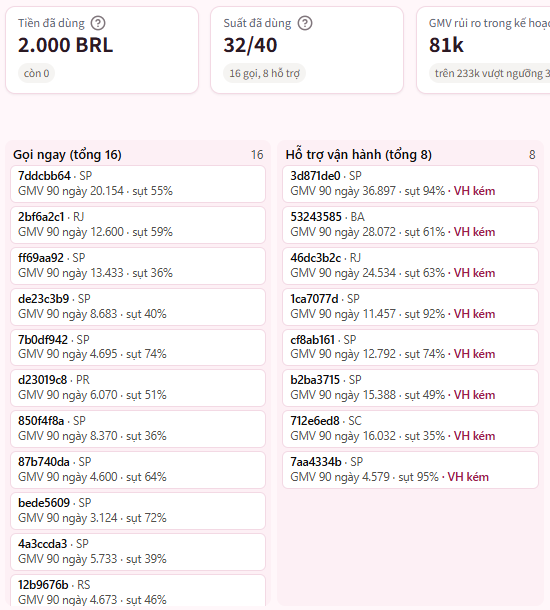
\includegraphics[width=0.47\textwidth]{image/app_7_crop_cols.png}}\hfill
\fbox{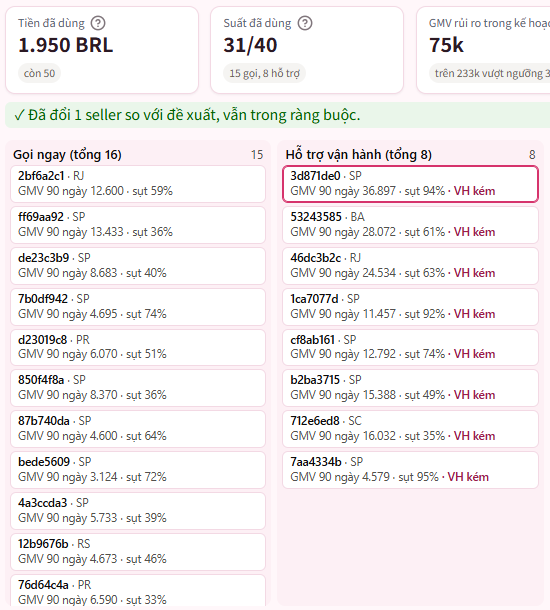
\includegraphics[width=0.47\textwidth]{image/app_8_crop_cols.png}}
\caption{Bảng kế hoạch mốc 01/03/2018 trước (trái) và sau (phải) khi kéo seller \texttt{7ddcbb64} khỏi cột \texttt{CALL}: tiền đã dùng giảm từ 2.000 xuống 1.950 BRL, số suất từ 32 xuống 31, và thanh xác nhận báo kế hoạch vẫn trong ràng buộc}
\label{fig:ui_drag}
\end{figure}

\appimage[0.7\textwidth]{image/app_9_bang_vuot_rang_buoc.png}{Cảnh báo khi thao tác tay vượt ngân sách (mốc 01/03/2018): nút Chốt kế hoạch bị khóa}{fig:ui_violate}

\appimage{image/app_5_kiem_chung.png}{Luồng A, bước 4 -- Kiểm chứng trên các tháng đã biết kết quả}{fig:ui_validation}

\appimage{image/app_4_whatif_tuyen.png}{Luồng B -- What-if hẹn giao theo tuyến}{fig:ui_whatif}
